% !TEX root = ../main.tex
\chapter{Kinematikk}
\label{Chapter:kinematikk}
\intro{En stor del av fysikken handler om å beskrive og forutsi posisjon og bevegelse for objekter (legemer). Kinematikk er læren om \textit{hvordan}legemer beveger seg. I kinematikken konsentrerer vi oss derfor om begreper som posisjon ($\vec{s}$), hastighet ($\vec{v}$) og akselerasjon ($\vec{a}$), som er verktøyene vi trenger for å beskrive bevegelse. Dette gir det rette grunnlaget for \textit{dynamikken} (/kraftlære), som kommer i neste kapittel, og handler om \textit{årsaken} legemers bevegelse.}

\spm{}{%
\item Hva er sammenhengen mellom posisjon, hastighet og akselerasjon?
\item Hvordan beskriver vi bevegelse med matematikk?
\item Hva er forskjellen på beskriven av bevegelse i 1 dimensjon og flere dimensjoner?}

\section{Hva er kinematikk?}
Kinematikk er studiet av hvordan objekter beveger seg, uten å vurdere (den mekaniske) årsaken til bevegelsen. For å bekrive dette effektivt er det spesielt tre begreper vi er ute etter, med hver sine forkortelser (i parentes):

\[\textrm{strekning ($\vec{s}$)}\quad,\quad\textrm{hastighet ($\vec{v}$)}\quad\textrm{og}\quad\textrm{akselerasjon ($\vec{a}$)}\]

Disse begrepene er alle sammen beskrevet som vektorer (derfor har de piler), ettersom de innbefatter konsepter som har både størrelse og retning. Sammen utgjør de verktøyene vi trenger for å kunne beskrive alt fra enkle scenario, slik som en ball som ruller ned en bakke og til mer kompliserte systemer, som planetenes bevegelse rundt solen. For å beskrive slike sammenhenger effektivt er det viktig å forstå relasjonene mellom strekning, fart og tid.

\section{Strekning ($\vec{s}$) og hastighet ($\vec{v}$)}
\begin{wrapfigure}[6]{r}[1.5cm]{3.6cm}
\vspace{-\baselineskip}%
\rotatebox{-15}{\href{https://youtu.be/nQ7h4B4D5ig?si=aB6griX7nAPx8UIF}{%
\begin{tikzpicture}[inner sep=0pt]
\node[anchor=south west] (thumb) at (0,0) {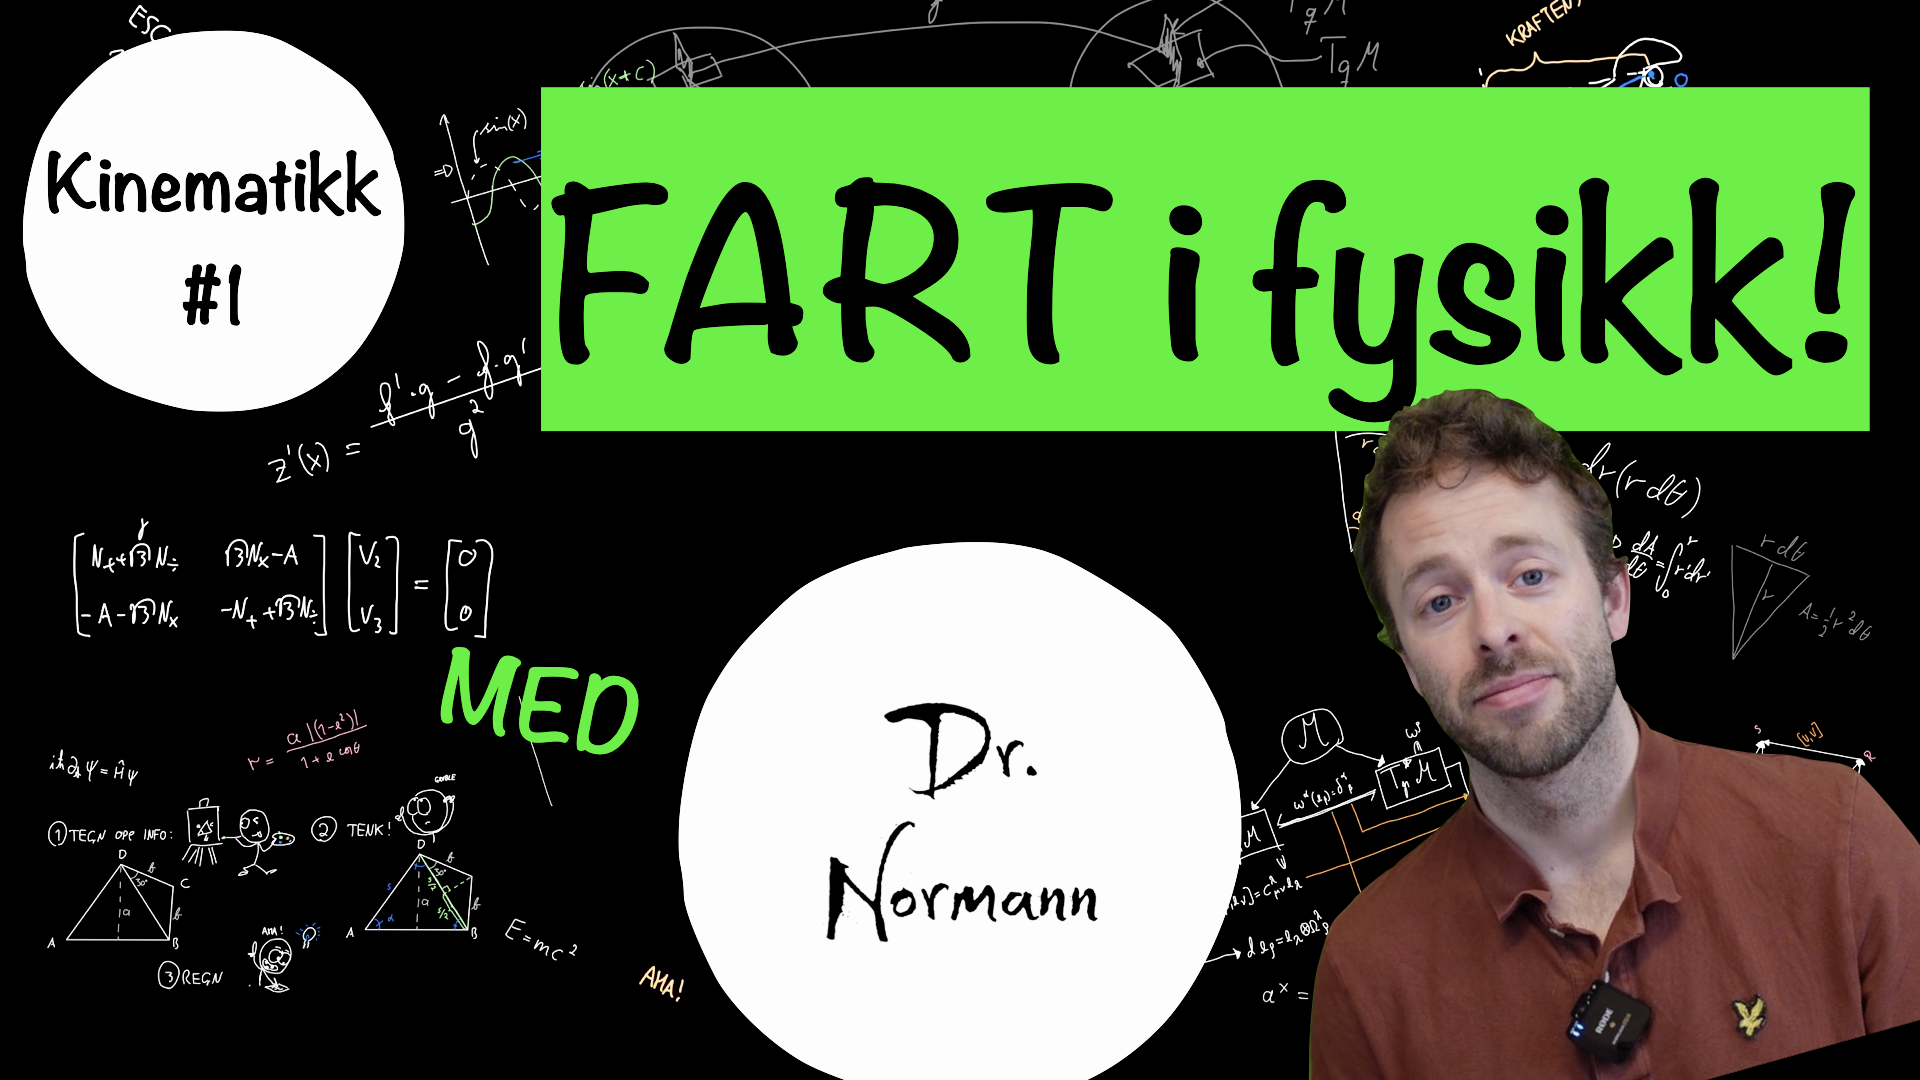
\includegraphics[width=3.6cm]{Images/YouTubeLenker/YT_FartIFysikk.png}};
\node[anchor=north west] at (thumb.south west) {
\includegraphics[width=1.2cm]{Images/YouTubeLenker/Icon.png}};
\end{tikzpicture}%
}}%
\end{wrapfigure}
Dersom all bevegelse er langs samme, rette linje så kallder vi bevegelsen \textit{rettlinjet}. I dette tilfellet kan vi beskrive strekning og fart som skalarer, altså uten vektornotasjon. Dersom bevegelsen er krum, må vi bruke vektorer. Dette refererer vi til som \textit{krumlinjet} bevegelse. Vi skal se på begge deler. Merk derfor følgende notasjon:
\begin{itemize}[itemsep=2pt, topsep=4pt, parsep=0pt]
    \item $s$ er strekning, altså størrelsen på \textbf{avstandsvektoren} $\vec{s}$. Vi kommer nok til å bruke begrep som \textit{posisjon} og \textit{forflytning} i tillegg til strekning og avstand. Poenget er at vi må gjøre forsljell på $s$ \textit{uten} vektortegn og \textit{med} vektortegn.
    \item $v$ kalles \textbf{fart} og er størrelsen på \textbf{hastighetsvektoren} $\vec{v}$.
    \item $a$ er størrelsen på \textbf{akselerasjonsvektoren} $\vec{a}$.
\end{itemize}

En bil som kjører på en rett strekning vekk fra en lyktestolpe tilbakelegger større og større strekning (målt fra lyktestolpen). Vi sier gjerne at strekningen er en funksjon av tid, og skriver $s(t)$:

\[s(t)=\textrm{strekning som funksjon av tid}.\]
% \vspace{-3em}
\begin{figure}[H]
    \centering
    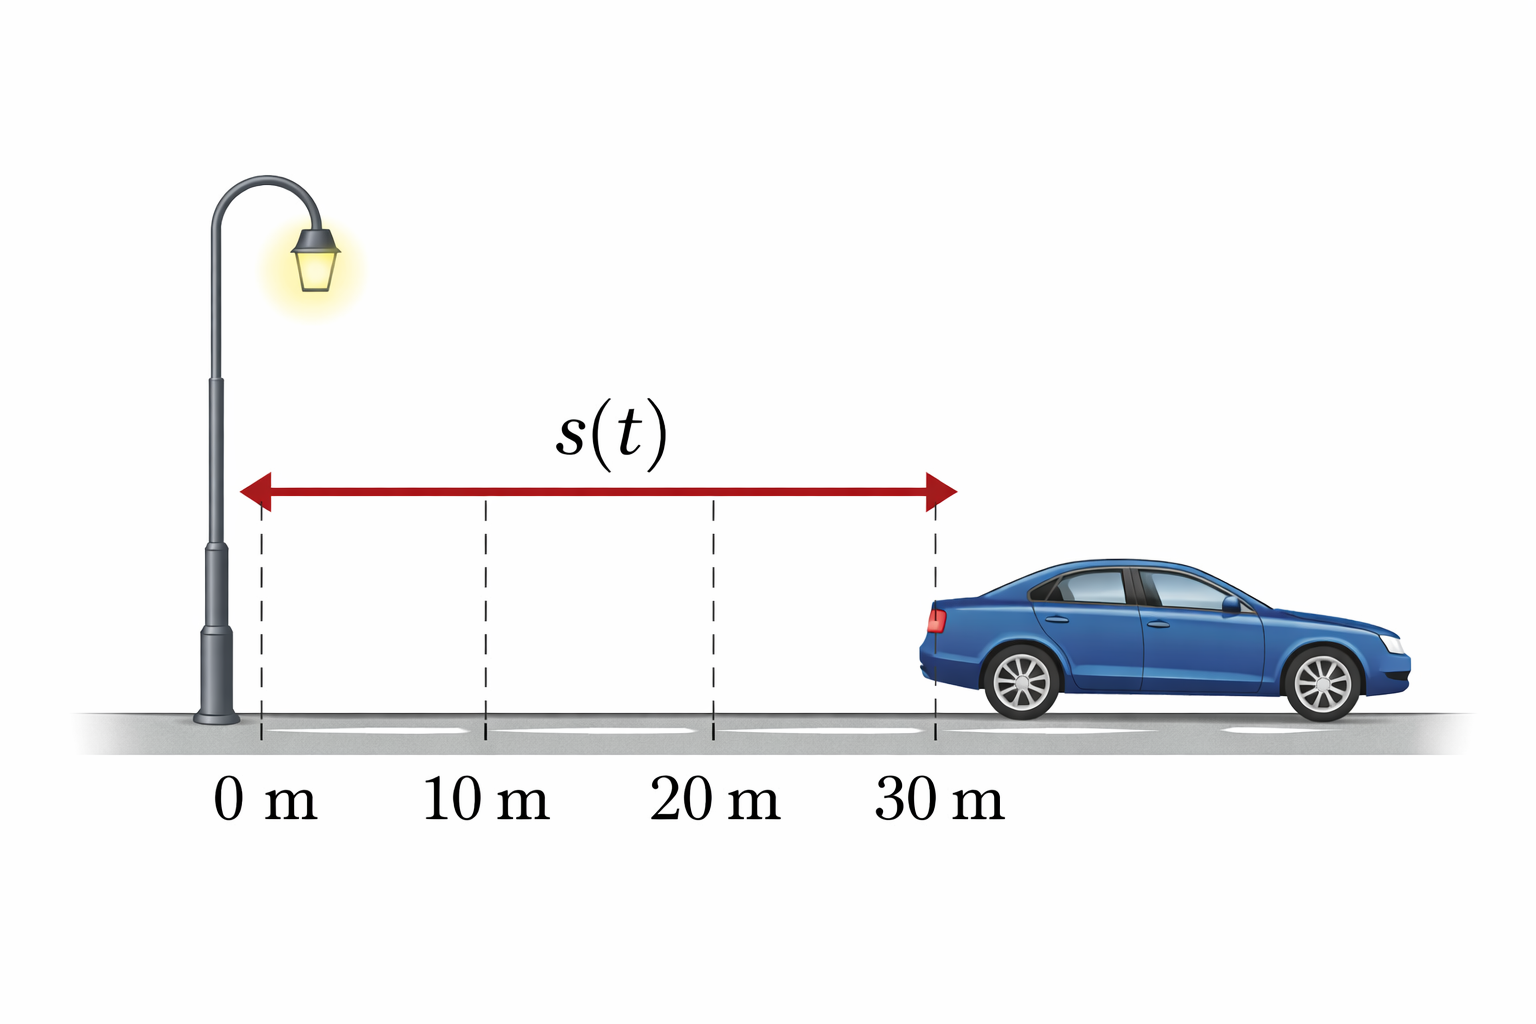
\includegraphics[width=0.7\linewidth, trim={0, 60mm, 0, 60mm},clip]{Images/Kapittel2:Kinematikk/Bil_fra_lyktestolpe.png}
    \caption{Eksempel på avstand mellom en lyktestolpe og forbipasserende bil.}
    \label{fig:fart strekning}
\end{figure}
% \vspace{-3em}
Vi kan illustrere beveglesen til bilen med grafer for fart og strekning. La oss anta at bilen holder konstant fart på $v=\SI{36}{\kilo\metre\per\hour}=\SI{10}{\metre\per\second}$. Da vil strekningen øke med 10 meter hvert sekund, og grafen for strekning vil være en rett linje som stiger jevnt. Grafen for fart vil være en horisontal linje på 10 m/s, siden farten ikke endrer seg. Dette er illustrert i figur \ref{fig:fart- og strekningsgrafer}.
\begin{figure}[H]
\centering
%--- Fartsgraf v(t) ----------------------------------------------------
% Plotområde 4.5 cm × 3.6 cm  |  x: 1.5 cm/s  |  y: 0.3 cm/(m/s), 0–12 m/s
\begin{subfigure}{0.48\textwidth}
  \centering
  \begin{tikzpicture}
    % Lys rutenett
    \foreach \xg in {1.5, 3.0, 4.5}{
      \draw[gray!25, thin] (\xg, 0) -- (\xg, 3.8);
    }
    \foreach \yg in {1.5, 3.0}{
      \draw[gray!25, thin] (0, \yg) -- (4.5, \yg);
    }
    % Akser
    \draw[->, thick] (-0.3, 0) -- (5.1, 0)
          node[right, font=\small] {Tid [s]};
    \draw[->, thick] (0, -0.3) -- (0, 4.4)
          node[above, font=\small] {Fart [m/s]};
    % Tidsaksen: strekmerker
    \foreach \xpos/\xlbl in {0/0, 1.5/1, 3.0/2, 4.5/3}{
      \draw[thin] (\xpos, 2.5pt) -- (\xpos, -2.5pt);
      \node[below=3pt, font=\scriptsize] at (\xpos, 0) {$\xlbl$};
    }
    % Fartsaksen: strekmerker
    \foreach \ypos/\ylbl in {0/0, 1.5/5, 3.0/10}{
      \draw[thin] (-2.5pt, \ypos) -- (2.5pt, \ypos);
      \node[left=4pt, font=\scriptsize] at (0, \ypos) {$\ylbl$};
    }
    % Konstant hastighet v = 10 m/s
    \draw[headCol, thick] (0, 3.0) -- (4.5, 3.0);
    \node[above right=2pt, headCol, font=\scriptsize]
          at (0, 3.0) {$v = 10\ \mathrm{m/s}$};
  \end{tikzpicture}
  \caption{Fartsgraf $v(t)$}
\end{subfigure}\hfill
%--- Posisjonsgraf s(t) ------------------------------------------------
% Plotområde 4.5 cm × 3.6 cm  |  x: 1.5 cm/s  |  y: 1.2 cm per 10 m, 0–30 m
\begin{subfigure}{0.48\textwidth}
  \centering
  \begin{tikzpicture}
    % Lys rutenett
    \foreach \xg in {1.5, 3.0, 4.5}{
      \draw[gray!25, thin] (\xg, 0) -- (\xg, 3.8);
    }
    \foreach \yg in {1.2, 2.4, 3.6}{
      \draw[gray!25, thin] (0, \yg) -- (4.5, \yg);
    }
    % Akser
    \draw[->, thick] (-0.3, 0) -- (5.1, 0)
          node[right, font=\small] {Tid [s]};
    \draw[->, thick] (0, -0.3) -- (0, 4.4)
          node[above, font=\small] {Strekning [m]};
    % Tidsaksen: strekmerker
    \foreach \xpos/\xlbl in {0/0, 1.5/1, 3.0/2, 4.5/3}{
      \draw[thin] (\xpos, 2.5pt) -- (\xpos, -2.5pt);
      \node[below=3pt, font=\scriptsize] at (\xpos, 0) {$\xlbl$};
    }
    % Strekningsaksen: strekmerker
    \foreach \ypos/\ylbl in {0/0, 1.2/10, 2.4/20, 3.6/30}{
      \draw[thin] (-2.5pt, \ypos) -- (2.5pt, \ypos);
      \node[left=4pt, font=\scriptsize] at (0, \ypos) {$\ylbl$};
    }
    % Posisjonslinje s = 10t
    \draw[headCol, thick] (0, 0) -- (4.5, 3.6);
    % Posisjonspunkter fra figur 3.1 (0 m, 10 m, 20 m, 30 m ved t = 0,1,2,3 s)
    \foreach \xpos/\ypos in {0/0, 1.5/1.2, 3.0/2.4, 4.5/3.6}{
      \fill[headCol] (\xpos, \ypos) circle(2.5pt);
    }
    % Kurve-etikett
    \node[above left=2pt, headCol, font=\scriptsize]
          at (2.5, 2.0) {$s = 10t$};
  \end{tikzpicture}
  \caption{Posisjonsgraf $s(t)$}
\end{subfigure}
\caption{Fart- og posisjonsgraf for bil som passerer lyktestolpe med
         konstant hastighet $v = 10\,\mathrm{m/s}$.}
\label{fig:fart- og strekningsgrafer}
\end{figure}

\begin{wrapfigure}[6]{l}[1.5cm]{3.6cm}
\vspace{-\baselineskip}%
\rotatebox{15}{\href{https://youtu.be/giCcfGv-uTc?si=0qJ3O-1g52nv1P7s}{%
\begin{tikzpicture}[inner sep=0pt]
\node[anchor=south west] (thumb) at (0,0) {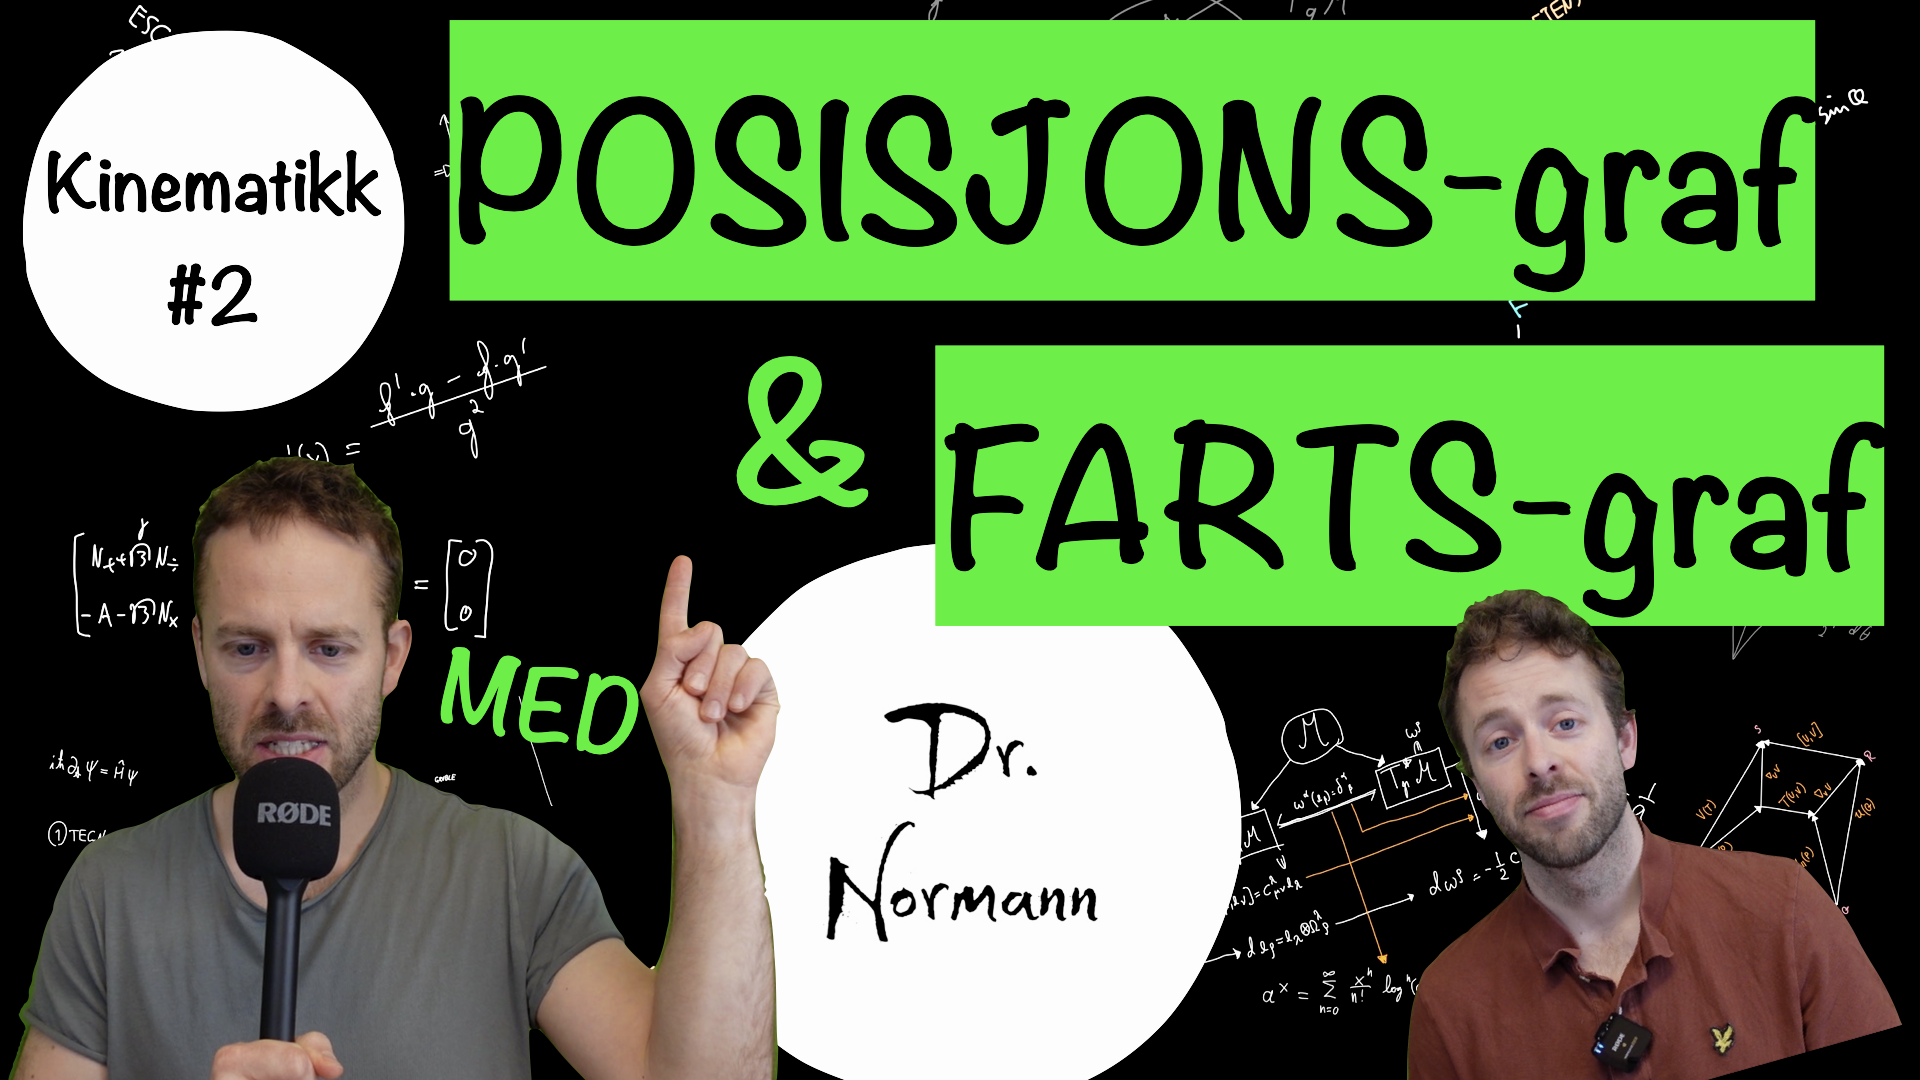
\includegraphics[width=3.6cm]{Images/YouTubeLenker/YT_PosisjonsOgFartsgraf.png}};
\node[anchor=north west] at (thumb.south west) {
\includegraphics[width=1.2cm]{Images/YouTubeLenker/Icon.png}};
\end{tikzpicture}%
}}%
\end{wrapfigure}
Stigningstallet til strekningsgrafen kan vi regne ut momentant ved derivasjon, eller som gjennomsnittet av endring i posisjon over en periode:
\begin{align*}
    \textrm{v} = \frac{\Delta\textrm{s}}{\Delta\textrm{t}} = \frac{\SI{10}{\metre}}{\SI{1}{\second}} = \SI{10}{\metre\per\second}
\end{align*}
Som vi kan se ut ifra grafene, er farten det samme som stigningstallet til strekningsgrafen. Fart er altså størrelsen som beskriver endring i posisjon, og uformelt skriver vi gjerne ``trekantformelen'' som mange alt har sett: 

\begin{align}
    v=\frac{s}{t}
\end{align}
\tanke{}{%
Hvordan måler man fart?}
Hvilken strekning er det snakk om i formelen over? Og hvilken tid? Når vi skal måle fart i fysikken, så er det alltid over et visst tidsrom, som vi gjerne kaller $\Delta t$. Det kan jo godt være at farten egentlig endret seg underveis i dette tidsrommet, uten at våre målinger fikk det med seg. Et eksempel kan være om du måler tiden Trine bruker på en 60-meter. La oss si at Trine bruker 12 sekunder. Da er den gjennomsnittlige farten hennes $\bar{v}=\SI{60}{\metre}/\SI{12}{\second}=\SI{5}{\metre\per\second}.$ Men det er jo ikke slik å forstå at Trine holdt samme fart hele løpet. I starten var farten gjerne 0m/s, mens den på slutten av løpet kanskje var 10 m/s. Det er derfor viktig å være klar over at når vi snakker om \textit{målt} fart, så handler det alltid om gjennomsnittsfart over et tidsintervall $\Delta t$. Tidsintervallene vi måler på kan være veldig små (slik som i et speedometer), men det er likefullt et gjennomsnitt over dette lille tidsintervallet. For å være litt mer presis definerer vi nå det vi kaller for \textit{gjennomsnittsfart}, som altså er lengden av \textit{gjennomsnittshastighets}-vektoren.

\defn{Gjennomsnittsfart og gjennomsnittshastighet}{
    Matematisk kan gjennomsnittshastigheten uttrykkes som:
    \begin{align}
        \bar{\vec{v}}= \frac{\vec{\Delta s}}{\Delta t}= \frac{\vec{s}(t+\Delta t) - \vec{s}(t)}{\Delta t}
    \end{align}
    hvor \( \Delta \vec{s} \) er den totale forflytningen, og \( \Delta t \) er den totale tiden. Lengden av denne vektoren kalles for gjennomsnittsfarten, og er gitt ved:
    \begin{align}
        \bar{v} = |\bar{\vec{v}}| = \frac{|\vec{\Delta s}|}{\Delta t}
    \end{align}
}
Gjennomsnitts\textit{fart} beskriver altså størrelsen på den totale forflytningen til et objekt delt på den totale tiden som har gått. Ettersom forflytning er en vektor, så er gjennomsnitts\textit{hastighet} en vektor. Gjennomsnittsfart er derimot en skalar, siden det er lengden av gjennomsnittshastighetsvektoren. 

\exm{Gjennomsnittsfart i rettlinjet bevegelse}{En bil kjører $\SI{60}{\kilo\metre}$ på $\SI{1.5}{\hour}$. Finn gjennomsnittsfarten i km/t. Gjør om til m/s
}
\svar{%
Vi bruker definisjonen $\bar{v} = \dfrac{\Delta s}{\Delta t}$:
\[\bar{v} = \frac{\SI{60}{\kilo\metre}}{\SI{1.5}{\hour}} = \doubleunderline{\SI{40}{\kilo\metre\per\hour}}\]
Vi bruker omregningsfaktoren $\SI{1}{\kilo\metre\per\hour} = \frac{\SI{1\,000}{\metre}}{\SI{3\,600}{\second}}$:
\[\bar{v} = 40\;\si{\kilo\metre\per\hour} \cdot \frac{\SI{1\,000}{\metre}}{\SI{3\,600}{\second}} = \frac{40\,000}{3\,600}\,\si{\metre\per\second} \approx \doubleunderline{\SI{11}{\metre\per\second}}\]
}

\oppgave{Gjennomsnittsfart i rettlinjet bevegelse}{%
En bil kjører $\SI{120}{\kilo\metre}$ på $\SI{1.5}{\hour}$.
\begin{enumerate}[a)]
    \item Finn gjennomsnittsfarten i km/t.
    \item Gjør om til m/s.
    \item En annen bil kjører samme strekning på $\SI{90}{\minute}$. Hvem kjørte raskest?
\end{enumerate}
}

\subsection*{Hastighet og fart i krumlinjet bevegelse} 
Når et objekt beveger seg krumlinjet, så kommer blir det hele litt mer komplisert enn ved rettlinjet bevegelse. Nå må vi nemlig ta høyde for at forflytningen $\Delta \vec{s}$ endrer retning. Se for deg en kurve gjennom rommet — la oss si det er banen som Erling Braut Haaland følger i en spurt. For ethvert par med tidspunkt så kan vi tegne opp en forskjellsvektor $\Delta\vec{s}$ som viser avstanden mellom posisjonen til Haaland ved de to tidspunktene. Denne vektoren kan vi bruke til å beregne gjennomsnittshastigheten til Haaland mellom de to tidspunktene. Kanskje ser du nå også at dersom vi lar $\Delta t$ gå mot null, så vil $\Delta\vec{s}$ også gå mot null, og vi vil kunne finne den momentane hastigheten til Haaland på et gitt tidspunkt. Denne hastigheten vil for et hvert tidspunkt være tangent til kurva som Haaland løper. Det er som en buss som er ute og kjører. Bussen sin lengde peker alltid i fartsretningen, og hadde vi tegnet en linje gjennom bussen så ville den linja til enhvert tid vært tangent til bussens bane.

%--- To figurer side om side: posisjonsvektorer (venstre) og hastighetsvektorer (høyre)
% Bezier: P0=(1.5,2.5), P1=(2.8,3.3), P2=(4.2,1.8), P3=(5.8,2.4)
% A (t=0.35): (2.906,2.683)  B (t=0.65): (4.189,2.353)  [verifisert]
% Tangenter (normalisert): t=0.20→(0.999,0.042), t=0.50→(0.963,-0.270), t=0.75→(0.994,-0.115)
\begin{figure}[ht!]
\centering

%=== VENSTRE: posisjonsvektorer og gjennomsnittshastighet ====================
\begin{minipage}[t]{0.52\textwidth}
\centering
\begin{tikzpicture}[font=\small, scale=1.0, >=stealth]

  %--- Origo ---------------------------------------------------------------
  \fill (0,0) circle(2.5pt);
  \node[below left=2pt] at (0,0) {$O$};

  %--- Kurven C ------------------------------------------------------------
  \draw[headCol, very thick]
    (1.5, 2.5) .. controls (2.8, 3.3) and (4.2, 1.8) .. (5.8, 2.4);
  \fill[headCol] (1.5, 2.5) circle(2pt);
  \node[headCol, left=5pt] at (1.5, 2.5) {$t=0$};
  \node[headCol, above right=2pt] at (5.55, 2.40) {$C$};

  %--- Punkt A = s(t) (t=0.35): (2.906, 2.683) ----------------------------
  \fill[defscol] (2.906, 2.683) circle(3pt);

  %--- Punkt B = s(t+Δt) (t=0.65): (4.189, 2.353) -------------------------
  \fill[oppsumcol] (4.189, 2.353) circle(3pt);

  %--- Posisjonsvektor s(t) ------------------------------------------------
  \draw[->, thick, defscol] (0,0) -- (2.906, 2.683)
        node[midway, above left=1pt] {$\vec{s}(t)$};

  %--- Posisjonsvektor s(t+Δt) ---------------------------------------------
  \draw[->, thick, oppsumcol] (0,0) -- (4.189, 2.353)
        node[midway, below right=1pt] {$\vec{s}(t{+}\Delta t)$};

  %--- Differansevektor Δs(t) ----------------------------------------------
  \draw[->, very thick, black!65, dashed] (2.906, 2.683) -- (4.189, 2.353);
  \node[font=\small] (dslabel) at (3.548, 2.90) {$\Delta\vec{s}(t)$};

  %--- Formel for gjennomsnittshastighet -----------------------------------
  \node[draw, rounded corners=3pt, fill=white, inner sep=5pt]
        (formula) at (2.6, 4.5)
        {$\bar{\vec{v}} = \dfrac{\Delta\vec{s}(t)}{\Delta t}$};

  %--- Pil fra etiketten opp til formelen ----------------------------------
  \draw[->, thin, black!50]
        (dslabel.north) to[out=90, in=270] (formula.south);

\end{tikzpicture}
\caption{Posisjonsvektorene $\vec{s}(t)$ og $\vec{s}(t{+}\Delta t)$ peker fra origo $O$ til to posisjoner på Haalands løpebane $C$. Forflytningsvektoren $\Delta\vec{s}(t)$ gir gjennomsnittshastigheten $\bar{\vec{v}} = \Delta\vec{s}(t)/\Delta t$ over tidsintervallet.}
\label{fig:haaland-pos}
\end{minipage}%
\hfill
%=== HØYRE: hastighetsvektorer langs banen ===================================
\begin{minipage}[t]{0.44\textwidth}
\centering
\begin{tikzpicture}[font=\small, scale=1.0, >=stealth]

  %--- Phantom: same bounding box som venstre figur (y=0 til y≈4.9) --------
  \path (0,0);
  \node[opacity=0] at (3.5, 4.9) {$x$};

  %--- Kurven C (samme Bezier) ---------------------------------------------
  \draw[headCol, very thick]
    (1.5, 2.5) .. controls (2.8, 3.3) and (4.2, 1.8) .. (5.8, 2.4);
  \fill[headCol] (1.5, 2.5) circle(2pt);
  \node[headCol, left=5pt] at (1.5, 2.5) {$t=0$};
  \node[headCol, above right=2pt] at (5.55, 2.40) {$C$};

  %--- v(t₁): pos=(2.293,2.739), dir=(0.999,0.042), l=0.60 ----------------
  % endpoint: (2.892, 2.764)
  \fill[defscol] (2.293, 2.739) circle(3pt);
  \node[below=3pt, font=\scriptsize] at (2.293, 2.739) {$t_1$};
  \draw[->, very thick, defscol] (2.293, 2.739) -- (2.892, 2.764)
        node[right=2pt] {$\vec{v}(t_1)$};

  %--- v(t₂): pos=(3.538,2.525), dir=(0.963,-0.270), l=0.90 ---------------
  % endpoint: (4.405, 2.282)
  \fill[defscol] (3.538, 2.525) circle(3pt);
  \node[below=3pt, font=\scriptsize] at (3.538, 2.525) {$t_2$};
  \draw[->, very thick, defscol] (3.538, 2.525) -- (4.405, 2.282)
        node[right=2pt] {$\vec{v}(t_2)$};

  %--- v(t₃): pos=(4.636,2.275), dir=(0.994,-0.115), l=1.10 ---------------
  % endpoint: (5.729, 2.148)
  \fill[defscol] (4.636, 2.275) circle(3pt);
  \node[below=3pt, font=\scriptsize] at (4.636, 2.275) {$t_3$};
  \draw[->, very thick, defscol] (4.636, 2.275) -- (5.729, 2.148)
        node[right=2pt] {$\vec{v}(t_3)$};

\end{tikzpicture}
\caption{Hastighetsvektorene $\vec{v}(t_1)$, $\vec{v}(t_2)$ og $\vec{v}(t_3)$ er tangenter til Haalands løpebane ved tre tidspunkter. Lengre piler indikerer at farten øker gjennom spurten.}
\label{fig:haaland-vel}
\end{minipage}

\end{figure}


I krumlinjet bevegelse er ikke nødvendigvis gjennomsnittsfart lenger et så nyttig begrep, da det ikke nødvendigvis gir et riktig inntrykk av hvor fort et legeme faktisk har beveget seg. For eksempel, hvis et objekt beveger seg i en sirkel og returnerer til utgangspunktet, vil den totale forflytningsvektoren være null (prøv å tegne opp $\Delta s$ mellom start og slutt!) --- og dermed er både gjennomsnittshastigheten \emph{og} gjennomsnittsfarten null. Men jeg er ganske sikker på at Karsten Warholm har løpt ganske fort rundt friidrettsbanen selv om gjennomsnittsfarten hans er null... Problemet oppstår fordi hastighet er definert ut ifra forflytningsvektoren $\vec{Delta s}$. Dermed får også farten, som er størrelsen på hastighetsvektoren, det samme problemet. Det er derfor nyttig å innføre et begrep til, kalt \textit{banefart}. Dette er farten som et legeme har til enhver tid langs den buen, eller banen, det går.

\defn{Banefart}{
    Banefarten $v$ er strekning tilbakelagt i en bane, dividert med tiden brukt på strekningen.
}
Her ser vi altså ikke på netto forflytning, men summativ forflytning. Merk at vi bruker samme synbol som ellers (for fart). Så får vi heller la sammenhengen gjøre det klart hvilket begrep som er hensiktsmessig å bruke. La oss ta et par eksempler som illustrerer forskjellen.

\exm{Båt på havet}{To båter skal seile fra punkt $P$ til punkt $R$. Båt 1 seiler i en rett linje fra $P$ til $R$ og bruker 2 timer på seilasen. Båt 2 seiler først 3 km øst til punktet $Q$ og deretter 4 km nord fra $Q$ til $R$. Den bruker 1 time på seilasen øst og 1 time på seilasen nord.\\
\textbf{a)} Skriv ned avstandsvektorene $\vec{\Delta s}_\text{PQ}$, $\vec{\Delta s}_\text{QR}$ og $\vec{\Delta s}_\text{PR}$ som beskriver de relevante forflytningene.\\
\textbf{b)} Bruk svarene fra a) til å skrive ned tilhørende hastighetsvektorer $\vec{v}_\text{PQ}$, $\vec{v}_\text{QR}$ og $\vec{v}_\text{PR}$. \\
\textbf{c)} Hva er gjennomsnittsfarten til båt 1 (lengden av hastighetsvektoren)?\\
\textbf{d)} Hva er gjennomsnittsfarten til båt 2 på hver av de to delstrekningene? Hva er den totale gjennomsnittsfarten til båt 2?\\
\textbf{e)} Hva er banefarten til båt 2 på hele strekningen?
}

\svar{%
\begin{center}
  \begin{tikzpicture}
    % Kompassindikator
    \draw[->,thin,gray!60](0.2,4.2)--(0.2,4.8)
          node[above,font=\scriptsize]{N};
    \draw[->,thin,gray!60](0.2,4.2)--(0.8,4.2)
          node[right,font=\scriptsize]{Ø};
    % Østlig etappe
    \draw[->,thick,headCol](0,0)--(3,0)
          node[midway,below=4pt,font=\small]{$\SI{3}{\kilo\metre}$};
    % Nordlig etappe
    \draw[->,thick,defscol](3,0)--(3,4)
          node[midway,right=4pt,font=\small]{$\SI{4}{\kilo\metre}$};
    % Forflytningsvektor
    \draw[->,very thick,oppsumcol](0,0)--(3,4)
          node[midway,above left=2pt,font=\small]{$\vec{\Delta s}_{PR}=\SI{5}{\kilo\metre}$};
    % Rett vinkel
    \draw (3,0)++(-0.22,0)--++(0,0.22)--++(0.22,0);
    % Punkter
    \fill(0,0) circle(2pt) node[below left=2pt,font=\small]{$P$};
    \fill(3,0) circle(2pt) node[below right=2pt,font=\small]{$Q$};
    \fill[oppsumcol](3,4) circle(2pt) node[above right=1pt,font=\small]{$R$};
  \end{tikzpicture}
\end{center}

\begin{enumerate}[\textbf{\alph*)}]
    \item Forflytningsvektorene (se figur):
          \[\vec{\Delta s}_{PQ}=[3,\;0]\,\si{\kilo\metre},\quad
            \vec{\Delta s}_{QR}=[0,\;4]\,\si{\kilo\metre},\quad
            \vec{\Delta s}_{PR}=[3,\;4]\,\si{\kilo\metre}\]
    \item Hastighetsvektorene finner vi ved å dele hver forflytning på tiden som ble brukt på den etappen:
          \[\vec{v}_{PQ}=\frac{\vec{\Delta s}_{PQ}}{\SI{1}{\hour}}=[3,\;0]\,\si{\kilo\metre\per\hour},\quad
            \vec{v}_{QR}=\frac{\vec{\Delta s}_{QR}}{\SI{1}{\hour}}=[0,\;4]\,\si{\kilo\metre\per\hour}\]
          \[\vec{v}_{PR}=\frac{\vec{\Delta s}_{PR}}{\SI{2}{\hour}}=[1.5,\;2]\,\si{\kilo\metre\per\hour}\]
    \item Båt 1 seiler direkte fra $P$ til $R$, så gjennomsnittsfarten er nettopp lengden av $\vec{v}_{PR}$ fra b):
          \[\bar{v}_1=|\vec{v}_{PR}|=\sqrt{1.5^2+2^2}= \doubleunderline{\SI{2.5}{\kilo\metre\per\hour}}\]
    \item Gjennomsnittsfart per etappe for båt 2 er lengden av de tilhørende hastighetsvektorene fra b):
          \[\bar{v}_{PQ}=|\vec{v}_{PQ}|=\SI{3}{\kilo\metre\per\hour},\quad\bar{v}_{QR}=|\vec{v}_{QR}|=\SI{4}{\kilo\metre\per\hour}\]
          Den \emph{totale} gjennomsnittsfarten regnes derimot fra totalforflytningen over hele tiden --- altså igjen lengden av $\vec{v}_{PR}$:
          \[\bar{v}_2=|\vec{v}_{PR}|= \doubleunderline{\SI{2.5}{\kilo\metre\per\hour}}\]
          Selv om båt 2 hadde ulik fart på de to etappene, er den totale gjennomsnittsfarten altså identisk med båt 1. Gjennomsnittsfart avhenger kun av total forflytning og total tid --- ikke av hvordan farten varierte underveis. Vi ser at det er ikke denne farten vi er interessert i. Det egentlig interessante fartsbegrepet i akkurat denne sammenheng, er banefarten, som vi ser på i neste deloppgave.
    \item Den gjennomsnittlige banefarten ser i stedet på hvor langt båt 2 faktisk har seilt, uavhengig av retning:
          \[
          v_{\text{bane},2}=\frac{\SI{3}{\kilo\metre}+\SI{4}{\kilo\metre}}{\SI{2}{\hour}}= \doubleunderline{\SI{3.5}{\kilo\metre\per\hour}},
          \]
          altså høyere enn gjennomsnittsfarten på $\SI{2.5}{\kilo\metre\per\hour}$ --- nettopp fordi båt 2 seilte en lengre vei enn den rette linja fra $P$ til $R$. 
\end{enumerate}
}

Fra eksemplet over, med båtene, ser vi at når vi ikke lenger har en rettlinjet bevegelse, så er det nødvendig med en presisering. Vi må skille mellom total forflytning og strekning. Forflytning er en vektor som beskriver endring i posisjon, mens strekning er en skalar som beskriver hvor langt et objekt faktisk har beveget seg, om vi summerer forflytninger langs banen.  Dette er spesielt viktig når vi skal regne ut gjennomsnittsfart, da den avhenger av forflytningen, mens gjennomsnittlig banefart avhenger av strekningen.

\exm{Karsten Warholm}{Se for deg at Karsten Warholm løper med konstant fart gjennom en sving. Etter 7 sekunder har han løpt fra inngangen av svingen (punkt $P$) til midten (punkt $Q$). Radiusen i svingen er 36 meter.\\
\textbf{a)} Finn $\vec{\Delta s}$ mellom punktene $P$ og $Q$ og beregn gjennomsnittshastigheten og gjennomsnittsfarten på forflytningen $PQ$.\\
\textbf{b)} Beregn banefarten til Karsten gjennom svingen, når du vet at han egentlig løper en kvart sirkelbane.}

\svar{%
\begin{center}
  \begin{tikzpicture}[scale=0.9]
    % Bane: kvartssirkel fra P=(2.5,0) til Q=(0,2.5)
    \draw[headCol,thick](2.5,0) arc(0:90:2.5);
    % Stiplede radier
    \draw[dashed,gray!60](0,0)--(2.5,0)
          node[midway,below=3pt,font=\scriptsize]{$r{=}\SI{36}{\metre}$};
    \draw[dashed,gray!60](0,0)--(0,2.5);
    % Rett vinkel ved sentrum
    \draw(0.22,0)--++(0,0.22)--++(-0.22,0);
    % Forflytningsvektor (korde P til Q)
    \draw[->,very thick,oppsumcol](2.5,0)--(0,2.5)
          node[midway,right=4pt,font=\small]{$\vec{\Delta s}$};
    % Hastighetspiler (tangenter til banen)
    \draw[->,thick,defscol](2.5,0)--(2.5,0.85)
          node[right,font=\scriptsize]{$\vec{v}_P$};
    \draw[->,thick,defscol](0,2.5)--(-0.85,2.5)
          node[above,font=\scriptsize]{$\vec{v}_Q$};
    % Punkter og etiketter
    \fill[headCol](2.5,0) circle(2pt)
          node[below right=1pt,font=\small]{$P$};
    \fill[headCol](0,2.5) circle(2pt)
          node[above left=1pt,font=\small]{$Q$};
    \fill(0,0) circle(1.5pt);
  \end{tikzpicture}
\end{center}

\begin{enumerate}[\textbf{\alph*)}]
  \item Vi legger origo i sentrum av svingen, med $P$ på $x$-aksen og $Q$ på $y$-aksen, slik at $P=(36,\,0)\,\si{\metre}$ og $Q=(0,\,36)\,\si{\metre}$. Forflytningsvektoren fra $P$ til $Q$ blir da:
        \[\vec{\Delta s}_{PQ}=Q-P=\doubleunderline{[-36,\;36]\,\si{\metre}}\]
        med størrelse
        \[|\vec{\Delta s}_{PQ}|=\sqrt{36^2+36^2}=36\sqrt{2}\approx \underline{\SI{50.9}{\metre}}.\]
        Gjennomsnittshastigheten er forflytningen delt på tiden:
        \[\vec{\bar{v}}=\frac{\vec{\Delta s}_{PQ}}{\SI{7}{\second}}\approx \doubleunderline{[-5.14,\;5.14]\,\si{\metre\per\second}}\]
        og gjennomsnittsfarten er størrelsen på denne vektoren:
        \[\bar{v}=|\vec{\bar{v}}|=\frac{|\vec{\Delta s}_{PQ}|}{\SI{7}{\second}}\approx \doubleunderline{\SI{7.3}{\metre\per\second}}\]
        Dette virker påfallende lavt til å beskrive en toppidrettsutøver som spurter gjennom en sving --- vi undersøker hvorfor i b).
  \item Farten $|\vec{v}|$ til Karsten er konstant hele veien, men siden banen er krum, er strekningen han faktisk løper lengre enn forflytningen $|\vec{\Delta s}_{PQ}|$ fra a). Buelengden langs en kvart sirkel er:
        \[\Delta s=\tfrac{1}{4}\cdot 2\pi r=\tfrac{\pi\cdot 36}{2}=18\pi\approx \underline{\SI{56.5}{\metre}}\]
        Banefarten bruker denne strekningen --- altså hvor langt Karsten faktisk har løpt --- i stedet for forflytningen:
        \[v_{\text{bane}}=\frac{18\pi\,\si{\metre}}{\SI{7}{\second}}\approx \doubleunderline{\SI{8.1}{\metre\per\second}}\]
        Banefarten på $\SI{8.1}{\metre\per\second}$ er altså høyere enn gjennomsnittsfarten på $\SI{7.3}{\metre\per\second}$ fra a) --- nettopp fordi gjennomsnittsfarten kun ser på nettoforflytningen $PQ$, og ikke fanger opp at Karsten faktisk løper en lengre, krum bane. Gjennomsnittsfarten er derfor et dårlig mål på farten hans når tidsintervallet vi tar gjennomsnittet over, blir for stort.
\end{enumerate}
}
La oss tilslutt ta med et eksempel der vi vet retningen til en hastighetsvektor og skal finne komponentene. Denne type beregning så vi også på i forrige kapittel. 
\exm{Dekomponering av hastighet}{En fugl flyr med fart $v = \SI{15}{\metre\per\second}$ i en retning som utgjør $\theta = 37°$ over horisontalplanet ($\cos 37° \approx 0.80$, $\sin 37° \approx 0.60$).\\
\textbf{a)} Finn den horisontale komponenten $v_x$ og den vertikale komponenten $v_y$ av hastigheten.\\
\textbf{b)} Verifiser at $|\vec{v}| = \sqrt{v_x^2 + v_y^2} = \SI{15}{\metre\per\second}$.}

\svar{%
\noindent
\begin{minipage}[t]{0.55\linewidth}
  \vspace{0pt}
  \begin{enumerate}[\textbf{\alph*)}]
    \item Vi dekomponerer langs de to aksene (se figur):
          \[v_x = v\cos\theta = 15\cdot 0.80 = \doubleunderline{\SI{12}{\metre\per\second}}\]
          \[v_y = v\sin\theta = 15\cdot 0.60 = \doubleunderline{\SI{9}{\metre\per\second}}\]
    \item Pythagoras bekrefter:
          \[\sqrt{v_x^2+v_y^2}=\sqrt{12^2+9^2}=\sqrt{144+81}=\sqrt{225}= \doubleunderline{\SI{15}{\metre\per\second}}\;\checkmark\]
  \end{enumerate}
  Merk at dette er det samme $9$-$12$-$15$-trekantforholdet (skalert $3$-$4$-$5$) som dukket opp i eksempel 3.2, men nå brukt til å gå fra totalfart til komponenter.
\end{minipage}%
\hfill
\begin{minipage}[t]{0.40\linewidth}
  \vspace{0pt}
  \centering
  % Vektortrekant: v=15, vx=12, vy=9, theta=37°
  \begin{tikzpicture}[font=\small, scale=0.85]
    % Fylt trekant
    \fill[headCol!12](0,0)--(4,0)--(4,3)--cycle;
    % Horisontal komponent vx
    \draw[->,thick,defscol](0,0)--(4,0)
          node[midway,below=3pt]{$v_x=\SI{12}{\metre\per\second}$};
    % Vertikal komponent vy
    \draw[->,thick,oppsumcol](4,0)--(4,3)
          node[midway,right=3pt]{$v_y=\SI{9}{\metre\per\second}$};
    % Totalvektoren v
    \draw[->,very thick,headCol](0,0)--(4,3)
          node[midway,above left=2pt]{$v=\SI{15}{\metre\per\second}$};
    % Rett vinkel
    \draw(4,0)++(-0.28,0)--++(0,0.28)--++(0.28,0);
    % Vinkel theta
    \draw[thin](0.85,0) arc(0:36.87:0.85);
    \node[right=2pt,font=\scriptsize]at(0.80,0.22){$\theta$};
    % Origo
    \fill(0,0) circle(1.5pt);
  \end{tikzpicture}
\end{minipage}
}

\subsubsection{Momentanfart}
Fra eksemplet med de to båtene, samt Karsten Warholm, så ser vi at hva gjennomsnittsfarten beregner til å være, er veldig avhengig av hvor ofte vi måler. Desto kortere tidsintervall vi måler på, desto mer nøyaktig blir resultatet. I praksis kan vi ofte måle posisjonen til et legeme veldig ofte, og dermed kan vi finne ut hva farten er på et gitt tidspunkt. Dette kaller vi for \textit{momentanhastighet}. 

Momentanhastighet er hastigheten til et objekt på et spesifikt tidspunkt. Det beskriver hvor raskt et objekt beveger seg i akkurat det øyeblikket, og er derfor den ``øyeblikkelige'' hastigheten.

Geometrisk kan vi forstå dette ved å betrakte posisjonskurven $s(t)$: gjennomsnittsfarten over intervallet $[t_0,\,t_0+\Delta t]$ er stigningstallet til \textit{sekantlinjen} gjennom punktene $(t_0,\,s(t_0))$ og $(t_0+\Delta t,\,s(t_0+\Delta t))$. Lar vi $\Delta t \to 0$, vil sekantlinjen nærme seg \textit{tangentlinjen} ved $t_0$ (se figuren under). Stigningstallet til tangentlinjen er nettopp den deriverte, og vi skriver:
\[
  v(t_0)
  = \lim_{\Delta t \to 0} \frac{\Delta s}{\Delta t}
  = \frac{ds}{dt}\bigg|_{t=t_0}
\]

%--- Illustrasjon: sekantlinje → tangentlinje når Δt → 0 ---------------
% Kurve: s(t) = 0.2 t²
% P ved t₀=2.0  →  s=0.8,  tangentslope = 0.80
% Q ved t =4.5  →  s=4.05, sekant PQ slope = 1.30  (stiplet)
% R ved t =3.2  →  s=2.048, sekant PR slope = 1.04  (hel)
% Linjeetiketter: alle tre er plassert til høyre for kurvens slutt (x>4.65),
%                 i åpent felt, slik at de ikke skriver seg over tegningen.
% «Δt→0»: label øverst ved x=3.1, pil ned-venstre til (2.75, 2.75).
\begin{center}
\begin{tikzpicture}[scale=1.4, font=\small]
  %--- Akser ---
  \draw[->, thick] (-0.3, 0) -- (6.6, 0) node[right] {$t$};
  \draw[->, thick] (0, -0.3) -- (0, 4.9) node[above] {$s(t)$};
  %--- Posisjonskurve: s = 0.2t² ---
  \draw[headCol, thick, domain=0:4.65, samples=80]
    plot (\x, {0.2*\x*\x});
  %--- Fastpunkt P ---
  \fill[headCol] (2.0, 0.8) circle(2.5pt);
  \node[left=3pt] at (2.0, 0.8) {$P$};
  %--- Sekantlinje PQ (stor Δt) – stiplet, mørkere ---
  \draw[black!55, semithick, dashed]
    (1.4, {1.30*1.4-1.80}) -- (4.9, {1.30*4.9-1.80});
  \fill[black!55] (4.5, 4.05) circle(2pt);
  \node[above left=2pt, black!60, font=\scriptsize] at (4.5, 4.05) {$Q$};
  %--- Sekantlinje PR (liten Δt) – hel linje, lysere ---
  \draw[black!30, semithick]
    (1.3, {1.04*1.3-1.28}) -- (4.8, {1.04*4.8-1.28});
  \fill[black!36] (3.2, 2.048) circle(2pt);
  \node[right=3pt, black!42, font=\scriptsize] at (3.2, 2.048) {$R$};
  %--- Tangentlinje ved P – oransje, tykk ---
  \draw[oppsumcol, thick]
    (1.1, {0.8*1.1-0.8}) -- (5.3, {0.8*5.3-0.8});
  %--- Δt/Δs-trekant (prikket, svak) ---
  \draw[dotted, gray!65, thin] (2.0, 0.8) -- (4.5, 0.8)
        node[midway, below=2pt, gray!80, font=\scriptsize] {$\Delta t$};
  \draw[dotted, gray!65, thin] (4.5, 0.8) -- (4.5, 4.05)
        node[midway, right=2pt, gray!80, font=\scriptsize] {$\Delta s$};
  %--- t-akse-etiketter ---
  \draw[thin] (2.0, 2.5pt) -- (2.0, -2.5pt);
  \node[below=2pt, font=\scriptsize] at (2.0, 0) {$t_0$};
  \draw[thin] (4.5, 2.5pt) -- (4.5, -2.5pt);
  \node[below=2pt, font=\scriptsize] at (4.5, 0) {$t_0{+}\Delta t$};
  %--- Linjeetiketter: hver plassert forbi kurvens slutt, i åpent felt til høyre ---
  \node[right=3pt, black!60, font=\scriptsize]
        at (4.9, {1.30*4.9-1.80}) {sekant $PQ$};
  \node[right=3pt, black!42, font=\scriptsize]
        at (4.8, {1.04*4.8-1.28}) {sekant $PR$};
  \node[right=3pt, oppsumcol, font=\scriptsize]
        at (4.7, {0.8*4.7-0.8}) {tangentlinje};
  %--- Δt→0: label øverst, pil kurver ned-venstre til klart rom ---
  \draw[->, thin, black!45]
        (3.1, 4.7) to[out=245, in=95] (2.75, 2.75);
  \node[right=1pt, black!50, font=\scriptsize] at (3.1, 4.7)
        {$\Delta t \to 0$};
\end{tikzpicture}
\end{center}

\defn{Momentanhastighet}{
    Matematisk kan momentanfart finnes ved å ta den deriverte av posisjonen med hensyn til tid:
    \begin{align}
        \vec{v} &= \frac{d\vec{s}}{dt}
    \end{align}
    Dette gir oss hastigheten nøyaktig i det øyeblikket vi er interessert i.
}

\exm{Speedometer}{
Tenk deg at du kjører bil og ser på speedometeret. Hastigheten som vises på speedometeret er momentanhastigheten din. Den kan endre seg fra ett sekund til et annet hvis du akselererer eller bremser. \\

\textit{Metode:}
Momentanhastighet er hastigheten til et objekt på et spesifikt tidspunkt. I dette tilfellet viser speedometeret bilens hastighet i sanntid, som kan variere hvis du akselererer eller bremser. Speedometeret gir dermed en direkte måling av bilens momentanhastighet, som er et uttrykk for hvor raskt bilen beveger seg i akkurat det øyeblikket.
}

Den store forskjellen mellom momentanfart og gjennomsnittsfart er at momentanfart ser på hastigheten i et spesifikt øyeblikk, mens gjennomsnittsfart ser på den totale bevegelsen over tid. Momentanfarten kan variere kraftig under en bevegelse, mens gjennomsnittsfarten gir en enkel verdi som representerer hele perioden.

\exm{Momentanhastighet}{Posisjonen til en firhjuling på et jorde er gitt ved $vec{s}(t) = (2t^2, 3t)$ i meter og sekunder.\\
\textbf{a)} Vis at uttrykket for momentanhastigheten $\vec{v}(t)$ til firhjulingen er gitt ved $\vec{v}(t) = (4t, 3)$.\\
\textbf{b)} Hva er momentanhastigheten ved $t = \SI{2}{\second}$?\\
\textbf{c)} Ved hvilken tid er momentanhastigheten $\vec{v} = (16, 12)\,\si{\metre\per\second}$?

}

\oppgave{Momentanhastighet}{%
Et legeme beveger seg etter posisjonslikningen $s(t) = 3t^2 + 2t$ (i meter og sekunder).
\begin{enumerate}[a)]
    \item For den som kan derivere: Vis at momentanfarten er gitt ved $v(t) = 6t + 2$.
    \item Hva er momentanhastigheten ved $t = \SI{2}{\second}$?
    \item Ved hvilken tid er momentanfarten $v = \SI{20}{\metre\per\second}$?
\end{enumerate}
}

\svar{%
\begin{enumerate}[a)]
  \item Vi deriverer $s(t) = 3t^2 + 2t$ ledd for ledd med potensregelen
    $\frac{d}{dt}(t^n) = nt^{n-1}$:
    \[
      v(t) = \frac{ds}{dt} = 3 \cdot 2t^{2-1} + 2 \cdot 1 = 6t + \SI{2}{\metre\per\second}
      \quad\checkmark
    \]
  \item Vi setter inn $t = \SI{2}{\second}$:
    \[
      v(2) = 6 \cdot 2 + 2 = 12 + 2 = \doubleunderline{\SI{14}{\metre\per\second}}
    \]
  \item Vi løser likningen $v(t) = \SI{20}{\metre\per\second}$:
    \[
      6t + 2 = 20
      \implies 6t = 18
      \implies t = \doubleunderline{\SI{3}{\second}}
    \]
\end{enumerate}
}


\subsubsection{Konstant fart}
 Vi kan tilslutt merke oss at desom farten ikke endrer seg, men er konstant, da er \textit{momentanfarten} til enhver tid den samme som \textit{gjennomsnittsfarten}. Ved konstant hastighet vil den tilbakelagte distansen være proporsjonal med tiden som har gått.


\oppgave{Konstant hastighet}{%
En syklist kjører med konstant hastighet $v = \SI{8}{\metre\per\second}$.
\begin{enumerate}[a)]
    \item Hvor langt har syklisten kjørt etter $t = \SI{10}{\second}$?
    \item Hvor langt har syklisten kjørt etter $t = \SI{2}{\minute}$?
    \item Hvor lang tid tar det å tilbakelegge $s = \SI{2.0}{\kilo\metre}$?
\end{enumerate}
}

\oppgave{En oppgave til}{%
En båt beveger seg med fart $v=5.0$ knopp i Nord-Østlig retning. Finn farta i nordlig retning ($v_\text{N}$) og farta i østlig retning (($v_\text{Ø}$))
}




\section{Akselerasjon}
\begin{wrapfigure}[6]{r}[1.5cm]{3.6cm}
\vspace{-\baselineskip}%
\rotatebox{-15}{\href{https://youtu.be/Q4S15FxYehk?si=moOmoKIu3yFgQlFl}{%
\begin{tikzpicture}[inner sep=0pt]
\node[anchor=south west] (thumb) at (0,0) {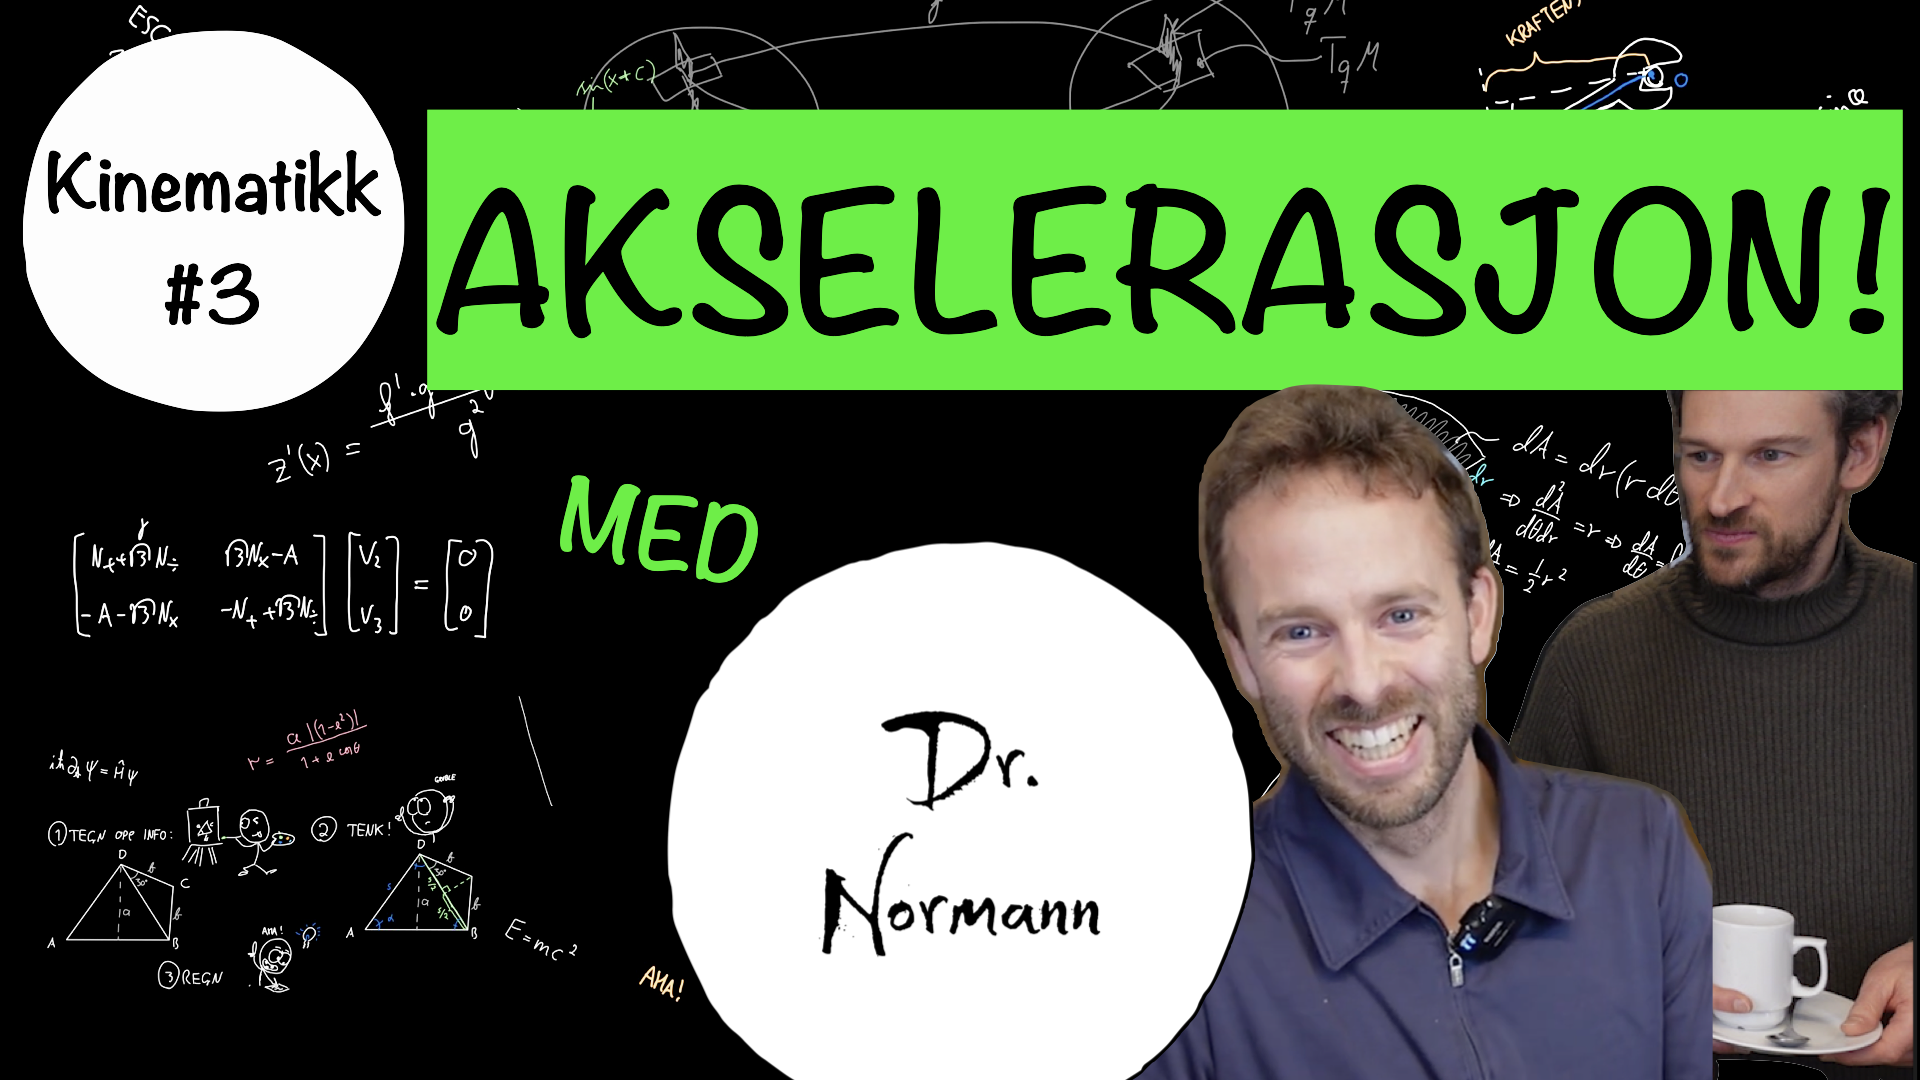
\includegraphics[width=3.6cm]{Images/YouTubeLenker/YT_Akselerasjon.png}};
\node[anchor=north west] at (thumb.south west) {
\includegraphics[width=1.2cm]{Images/YouTubeLenker/Icon.png}};
\end{tikzpicture}%
}}%
\end{wrapfigure}
Vi har så langt sett at endringen i strekning kalles fart. Men hva kalles endring i fart? Jo, det kalles \textit{akselerasjon}. Eller mer presist, så er akselerasjon et mål på endring i hastighet. Og hastighet har både størrelse og retning (er en vektor). Derfor handler akselerasjon om endring både av fartens størrelse og retning. Hvis akselerasjonen er positiv, øker objektets hastighet, mens en negativ akselerasjon (ofte kalt retardasjon, deselerasjon eller bare bremsing) betyr at hastigheten minker.
\tanke{}{%
Hva tenker du om størrelse og retning på akselerasjonen i følgende to tilfeller?\\
(I) En racerbil kjører med konstant fart på et rett strekke.\\
(II) En racerbil kjører med konstant fart gjennom en sving.
}



%--- Figur 3.3 og 3.4 side om side: konstant vs. varierende akselerasjon ----
% Figur 3.3: s₀=0, v₀=−2 m/s, a=1 m/s² (konstant)
%   s(t)=½t²−2t, v(t)=t−2, a(t)=1
% Figur 3.4: s₀=0, v₀=−2 m/s; a₁=2 m/s² for t∈[0,2 s], a₂=−1 m/s² for t∈[2,5 s]
%   Fase 1: v(t)=2t−2, s(t)=t²−2t
%   Fase 2: v(t)=4−t,  s(t)=2(t−2)−½(t−2)²
%   Kontrollpunkter: s(1)=−1, s(2)=0, s(4)=2(max), s(5)=1.5
%                    v(0)=−2, v(1)=0, v(2)=2, v(4)=0, v(5)=−1
% Skala (begge): x: 0.9 cm/s | y_s: 0.72 cm/m | y_v: 0.6 cm/(m/s) | y_a: 0.6 cm/(m/s²)
\begin{figure}[ht!]
\centering

%=== VENSTRE: Figur 3.3 – konstant akselerasjon ==========================
\begin{minipage}[t]{0.46\textwidth}
\centering

%--- Posisjonsgraf s(t) = ½t² − 2t ---
\begin{tikzpicture}
  \foreach \xg in {0.9, 1.8, 2.7, 3.6, 4.5}{
    \draw[gray!25, thin] (\xg, -1.6) -- (\xg, 2.0); }
  \foreach \yg in {-1.44, -0.72, 0.72, 1.44}{
    \draw[gray!25, thin] (0, \yg) -- (4.5, \yg); }
  \draw[->, thick] (-0.3, 0) -- (5.2, 0)
        node[right, font=\small] {$t$ [s]};
  \draw[->, thick] (0, -1.8) -- (0, 2.2)
        node[above, font=\small] {Posisjon [m]};
  \foreach \xpos/\xlbl in {0.9/1, 1.8/2, 2.7/3, 3.6/4, 4.5/5}{
    \draw[thin] (\xpos, 2.5pt) -- (\xpos, -2.5pt);
    \node[below=3pt, font=\scriptsize] at (\xpos, 0) {$\xlbl$}; }
  \foreach \ypos/\ylbl in {-1.44/{-2}, -0.72/{-1}, 0.72/1, 1.44/2}{
    \draw[thin] (-2.5pt, \ypos) -- (2.5pt, \ypos);
    \node[left=4pt, font=\scriptsize] at (0, \ypos) {$\ylbl$}; }
  \node[below left=1pt, font=\scriptsize] at (0, 0) {$0$};
  \draw[headCol, thick, domain=0:4.5, samples=60]
    plot (\x, {(4/9)*\x*\x - 1.6*\x});
  \node[above right=2pt, headCol, font=\scriptsize] at (3.6, 1.2) {$s(t)$};
\end{tikzpicture}

\smallskip

%--- Fartsgraf v(t) = t − 2 ---
\begin{tikzpicture}
  \foreach \xg in {0.9, 1.8, 2.7, 3.6, 4.5}{
    \draw[gray!25, thin] (\xg, -1.3) -- (\xg, 2.0); }
  \foreach \yg in {-1.2, -0.6, 0.6, 1.2, 1.8}{
    \draw[gray!25, thin] (0, \yg) -- (4.5, \yg); }
  \draw[->, thick] (-0.3, 0) -- (5.2, 0)
        node[right, font=\small] {$t$ [s]};
  \draw[->, thick] (0, -1.5) -- (0, 2.2)
        node[above, font=\small] {Fart [m/s]};
  \foreach \xpos/\xlbl in {0.9/1, 1.8/2, 2.7/3, 3.6/4, 4.5/5}{
    \draw[thin] (\xpos, 2.5pt) -- (\xpos, -2.5pt);
    \node[below=3pt, font=\scriptsize] at (\xpos, 0) {$\xlbl$}; }
  \foreach \ypos/\ylbl in {-1.2/{-2}, -0.6/{-1}, 0.6/1, 1.2/2, 1.8/3}{
    \draw[thin] (-2.5pt, \ypos) -- (2.5pt, \ypos);
    \node[left=4pt, font=\scriptsize] at (0, \ypos) {$\ylbl$}; }
  \node[below left=1pt, font=\scriptsize] at (0, 0) {$0$};
  \draw[headCol, thick] (0, -1.2) -- (4.5, 1.8);
  \node[above right=2pt, headCol, font=\scriptsize] at (3.5, 1.5) {$v(t)$};
\end{tikzpicture}

\smallskip

%--- Akselerasjonsgraf a(t) = 1 m/s² ---
\begin{tikzpicture}
  \foreach \xg in {0.9, 1.8, 2.7, 3.6, 4.5}{
    \draw[gray!25, thin] (\xg, 0) -- (\xg, 2.2); }
  \draw[gray!25, thin] (0, 1.2) -- (4.5, 1.2);
  \draw[->, thick] (-0.3, 0) -- (5.2, 0)
        node[right, font=\small] {$t$ [s]};
  \draw[->, thick] (0, -0.3) -- (0, 2.6)
        node[above, font=\small] {Akselerasjon [m/s\textsuperscript{2}]};
  \foreach \xpos/\xlbl in {0.9/1, 1.8/2, 2.7/3, 3.6/4, 4.5/5}{
    \draw[thin] (\xpos, 2.5pt) -- (\xpos, -2.5pt);
    \node[below=3pt, font=\scriptsize] at (\xpos, 0) {$\xlbl$}; }
  \foreach \ypos/\ylbl in {0/0, 1.2/1}{
    \draw[thin] (-2.5pt, \ypos) -- (2.5pt, \ypos);
    \node[left=4pt, font=\scriptsize] at (0, \ypos) {$\ylbl$}; }
  \draw[headCol, thick] (0, 1.2) -- (4.5, 1.2);
  \node[above right=2pt, headCol, font=\scriptsize]
        at (0, 1.2) {$a = 1\ \mathrm{m/s}^2$};
  \node[left=4pt, font=\scriptsize, opacity=0] at (0, 0) {$-2$};
\end{tikzpicture}

\caption{Posisjon, fart og akselerasjon ved \emph{konstant} akselerasjon
         ($s_0=0$, $v_0=-2\,\mathrm{m/s}$, $a=1\,\mathrm{m/s}^2$).}
\label{Konstant akselerasjon}
\end{minipage}%
%=== SKILLELINJE ==========================================================
\hspace{4pt}{\color{black!25}\rule[-10cm]{0.4pt}{10cm}}\hspace{4pt}%
%=== HØYRE: Figur 3.4 – varierende akselerasjon ===========================
% Fase 1 (0≤t≤2): a=2 → v=2t−2, s=t²−2t
%   TikZ s: y=(8/9)x²−1.6x  [verifisert: t=1→y=−0.72, t=2→y=0]
% Fase 2 (2≤t≤5): a=−1 → v=4−t, s=2(t−2)−½(t−2)²
%   TikZ s: y=1.6(x−1.8)−(4/9)(x−1.8)²  [verifisert: t=4→y=1.44, t=5→y=1.08]
\begin{minipage}[t]{0.46\textwidth}
\centering

%--- Posisjonsgraf – stykkvis parabolsk ---
\begin{tikzpicture}
  \foreach \xg in {0.9, 1.8, 2.7, 3.6, 4.5}{
    \draw[gray!25, thin] (\xg, -1.6) -- (\xg, 2.0); }
  \foreach \yg in {-0.72, 0.72, 1.44}{
    \draw[gray!25, thin] (0, \yg) -- (4.5, \yg); }
  % Faseskille
  \draw[gray!40, dashed, thin] (1.8, -1.6) -- (1.8, 2.0);
  \draw[->, thick] (-0.3, 0) -- (5.2, 0)
        node[right, font=\small] {$t$ [s]};
  \draw[->, thick] (0, -1.8) -- (0, 2.2)
        node[above, font=\small] {Posisjon [m]};
  \foreach \xpos/\xlbl in {0.9/1, 1.8/2, 2.7/3, 3.6/4, 4.5/5}{
    \draw[thin] (\xpos, 2.5pt) -- (\xpos, -2.5pt);
    \node[below=3pt, font=\scriptsize] at (\xpos, 0) {$\xlbl$}; }
  \foreach \ypos/\ylbl in {-0.72/{-1}, 0.72/1, 1.44/2}{
    \draw[thin] (-2.5pt, \ypos) -- (2.5pt, \ypos);
    \node[left=4pt, font=\scriptsize] at (0, \ypos) {$\ylbl$}; }
  \node[below left=1pt, font=\scriptsize] at (0, 0) {$0$};
  % Fase 1: s=t²−2t → y=(8/9)x²−1.6x
  \draw[headCol, thick, domain=0:1.8, samples=30]
    plot (\x, {(8/9)*\x*\x - 1.6*\x});
  % Fase 2: s=2(t−2)−½(t−2)² → y=1.6(x−1.8)−(4/9)(x−1.8)²
  \draw[headCol, thick, domain=1.8:4.5, samples=30]
    plot (\x, {1.6*(\x-1.8) - (4/9)*(\x-1.8)*(\x-1.8)});
  \node[above right=2pt, headCol, font=\scriptsize] at (3.2, 1.44) {$s(t)$};
  % Usynlig node for lik venstre margin som fig 3.3
  \node[left=4pt, font=\scriptsize, opacity=0] at (0, -1.44) {$-2$};
\end{tikzpicture}

\smallskip

%--- Fartsgraf – stykkvis lineær ---
% Fase 1: v=2t−2 → linje (0,−1.2)→(1.8,1.2)
% Fase 2: v=4−t  → linje (1.8,1.2)→(4.5,−0.6)
\begin{tikzpicture}
  \foreach \xg in {0.9, 1.8, 2.7, 3.6, 4.5}{
    \draw[gray!25, thin] (\xg, -1.3) -- (\xg, 2.0); }
  \foreach \yg in {-1.2, -0.6, 0.6, 1.2}{
    \draw[gray!25, thin] (0, \yg) -- (4.5, \yg); }
  % Faseskille
  \draw[gray!40, dashed, thin] (1.8, -1.5) -- (1.8, 2.2);
  \draw[->, thick] (-0.3, 0) -- (5.2, 0)
        node[right, font=\small] {$t$ [s]};
  \draw[->, thick] (0, -1.5) -- (0, 2.2)
        node[above, font=\small] {Fart [m/s]};
  \foreach \xpos/\xlbl in {0.9/1, 1.8/2, 2.7/3, 3.6/4, 4.5/5}{
    \draw[thin] (\xpos, 2.5pt) -- (\xpos, -2.5pt);
    \node[below=3pt, font=\scriptsize] at (\xpos, 0) {$\xlbl$}; }
  \foreach \ypos/\ylbl in {-1.2/{-2}, -0.6/{-1}, 0.6/1, 1.2/2}{
    \draw[thin] (-2.5pt, \ypos) -- (2.5pt, \ypos);
    \node[left=4pt, font=\scriptsize] at (0, \ypos) {$\ylbl$}; }
  \node[below left=1pt, font=\scriptsize] at (0, 0) {$0$};
  \draw[headCol, thick] (0, -1.2) -- (1.8, 1.2);   % fase 1
  \draw[headCol, thick] (1.8, 1.2) -- (4.5, -0.6); % fase 2
  \node[above right=2pt, headCol, font=\scriptsize] at (2.8, 0.8) {$v(t)$};
  % Usynlig node for lik venstre margin
  \node[left=4pt, font=\scriptsize, opacity=0] at (0, 1.8) {$3$};
\end{tikzpicture}

\smallskip

%--- Akselerasjonsgraf – stegfunksjon ---
% Fase 1 (0≤t<2): a=2  → y=1.2
% Fase 2 (2<t≤5): a=−1 → y=−0.6
\begin{tikzpicture}
  \foreach \xg in {0.9, 1.8, 2.7, 3.6, 4.5}{
    \draw[gray!25, thin] (\xg, -0.8) -- (\xg, 1.6); }
  \foreach \yg in {-0.6, 0.6, 1.2}{
    \draw[gray!25, thin] (0, \yg) -- (4.5, \yg); }
  % Faseskille
  \draw[gray!40, dashed, thin] (1.8, -0.8) -- (1.8, 1.6);
  \draw[->, thick] (-0.3, 0) -- (5.2, 0)
        node[right, font=\small] {$t$ [s]};
  \draw[->, thick] (0, -1.0) -- (0, 1.9)
        node[above, font=\small] {Akselerasjon [m/s\textsuperscript{2}]};
  \foreach \xpos/\xlbl in {0.9/1, 1.8/2, 2.7/3, 3.6/4, 4.5/5}{
    \draw[thin] (\xpos, 2.5pt) -- (\xpos, -2.5pt);
    \node[below=3pt, font=\scriptsize] at (\xpos, 0) {$\xlbl$}; }
  \foreach \ypos/\ylbl in {-0.6/{-1}, 0.6/1, 1.2/2}{
    \draw[thin] (-2.5pt, \ypos) -- (2.5pt, \ypos);
    \node[left=4pt, font=\scriptsize] at (0, \ypos) {$\ylbl$}; }
  \node[below left=1pt, font=\scriptsize] at (0, 0) {$0$};
  % Stegfunksjon
  \draw[headCol, thick] (0, 1.2)  -- (1.8, 1.2);   % a=2, fase 1
  \draw[headCol, thick] (1.8, 1.2) -- (1.8, -0.6); % hopp ned ved t=2
  \draw[headCol, thick] (1.8, -0.6) -- (4.5, -0.6);% a=−1, fase 2
  % Usynlig node for lik venstre margin som fig 3.3
  \node[left=4pt, font=\scriptsize, opacity=0] at (0, 0) {$-2$};
\end{tikzpicture}

\caption{Posisjon, fart og akselerasjon ved \emph{varierende} akselerasjon
         ($s_0=0$, $v_0=-2\,\mathrm{m/s}$; $a_1=2\,\mathrm{m/s}^2$ for
         $t\in[0,2\,\mathrm{s}]$ og $a_2=-1\,\mathrm{m/s}^2$ for $t\in[2,5\,\mathrm{s}]$).}
\label{Variabel akselerasjon}
\end{minipage}

\end{figure}

På samme vis som for fart, så definerer vi også for akselerasjon det vi kaller \textit{gjennomsnittsakselerasjon}, som altså handler om å måle hastighetsendring over et tidsintervall.

\defn{Gjennomsnittsakselerasjon}{
    Gjennomsnittsakselerasjonen over et tidsintervall $\Delta t$ er definert som endringen i hastighetsvektoren delt på tidsintervallet:
    \begin{align}
        \bar{\vec{a}} = \frac{\Delta \vec{v}}{\Delta t} = \frac{\vec{v}(t+\Delta t) - \vec{v}(t)}{\Delta t}
    \end{align}
    Størrelsen $|\bar{\vec{a}}|$ kalles gjennomsnittlig akselerasjon, og enheten er m/s$^2$.
}
\textit{Momentanakselerasjonen} er da grenseverdien av gjennomsnittsakselerasjonen når tidsintervallet $\Delta t$ går mot null. Dette gir oss den eksakte akselerasjonen i et spesifikt øyeblikk, og kan uttrykkes som den deriverte av hastighetsvektoren med hensyn til tid, eller den andrederiverte av posisjonsvektoren med hensyn til tid.
\defn{Momentanakselerasjon}{
    Momentanakselerasjonen er grenseverdien av gjennomsnittsakselerasjonen når $\Delta t \to 0$, det vil si den deriverte av hastighetsvektoren – eller den andrederiverte av posisjonsvektoren – med hensyn til tid:
    \begin{align}
        \vec{a} = \lim_{\Delta t \to 0}\frac{\Delta \vec{v}}{\Delta t} = \frac{d\vec{v}}{dt} = \frac{d^2\vec{s}}{dt^2}
    \end{align}
    Akselerasjonen er altså en vektor: den har både størrelse og retning. I figurene \ref{Konstant akselerasjon} og \ref{Variabel akselerasjon} kan vi lese av akselerasjonen som stigningstallet til $v(t)$-kurven.
}

Figurene \ref{Konstant akselerasjon} og \ref{Variabel akselerasjon} illustrerer sammenhengen mellom strekning, fart og akselerasjon godt.I hvert panel viser øverste graf posisjonen $s(t)$, midterste graf farten $v(t)$, og nederste graf akselerasjonen $a(t)$. Legg merke til at fartsgrafens stigningstall til enhver tid tilsvarer verdien på akselerasjonsgrafen, og at posisjonsgrafens stigningstall tilsvarer verdien på fartsgrafens graf – slik det følger av derivasjonsrelasjonen.

\paragraph{Konstant akselerasjon}Når akselerasjonen er konstant, vil gjennomsnittsakselerasjon og momentanakselerasjon være identiske. 


\oppgave{Akselerasjon}{%
En bil øker farten fra $v_0 = \SI{20}{\metre\per\second}$ til $v = \SI{30}{\metre\per\second}$ på $\Delta t = \SI{5}{\second}$.
\begin{enumerate}[a)]
    \item Finn gjennomsnittsakselerasjonen.
    \item Er akselerasjonen positiv eller negativ? Hva betyr det?
    \item Dersom akselerasjonen er konstant, hva er farten etter ytterligere $\SI{3}{\second}$?
\end{enumerate}
}

\section{Bevegelseslikningene for konstant akselerasjon}
\label{sec:bevegelseslikninger}
\begin{wrapfigure}[6]{r}[1.5cm]{3.6cm}
\vspace{-\baselineskip}%
\rotatebox{-15}{\href{https://youtu.be/1rukKt6DYr0?si=_VYs_IJjoUBEMODn}{%
\begin{tikzpicture}[inner sep=0pt]
\node[anchor=south west] (thumb) at (0,0) {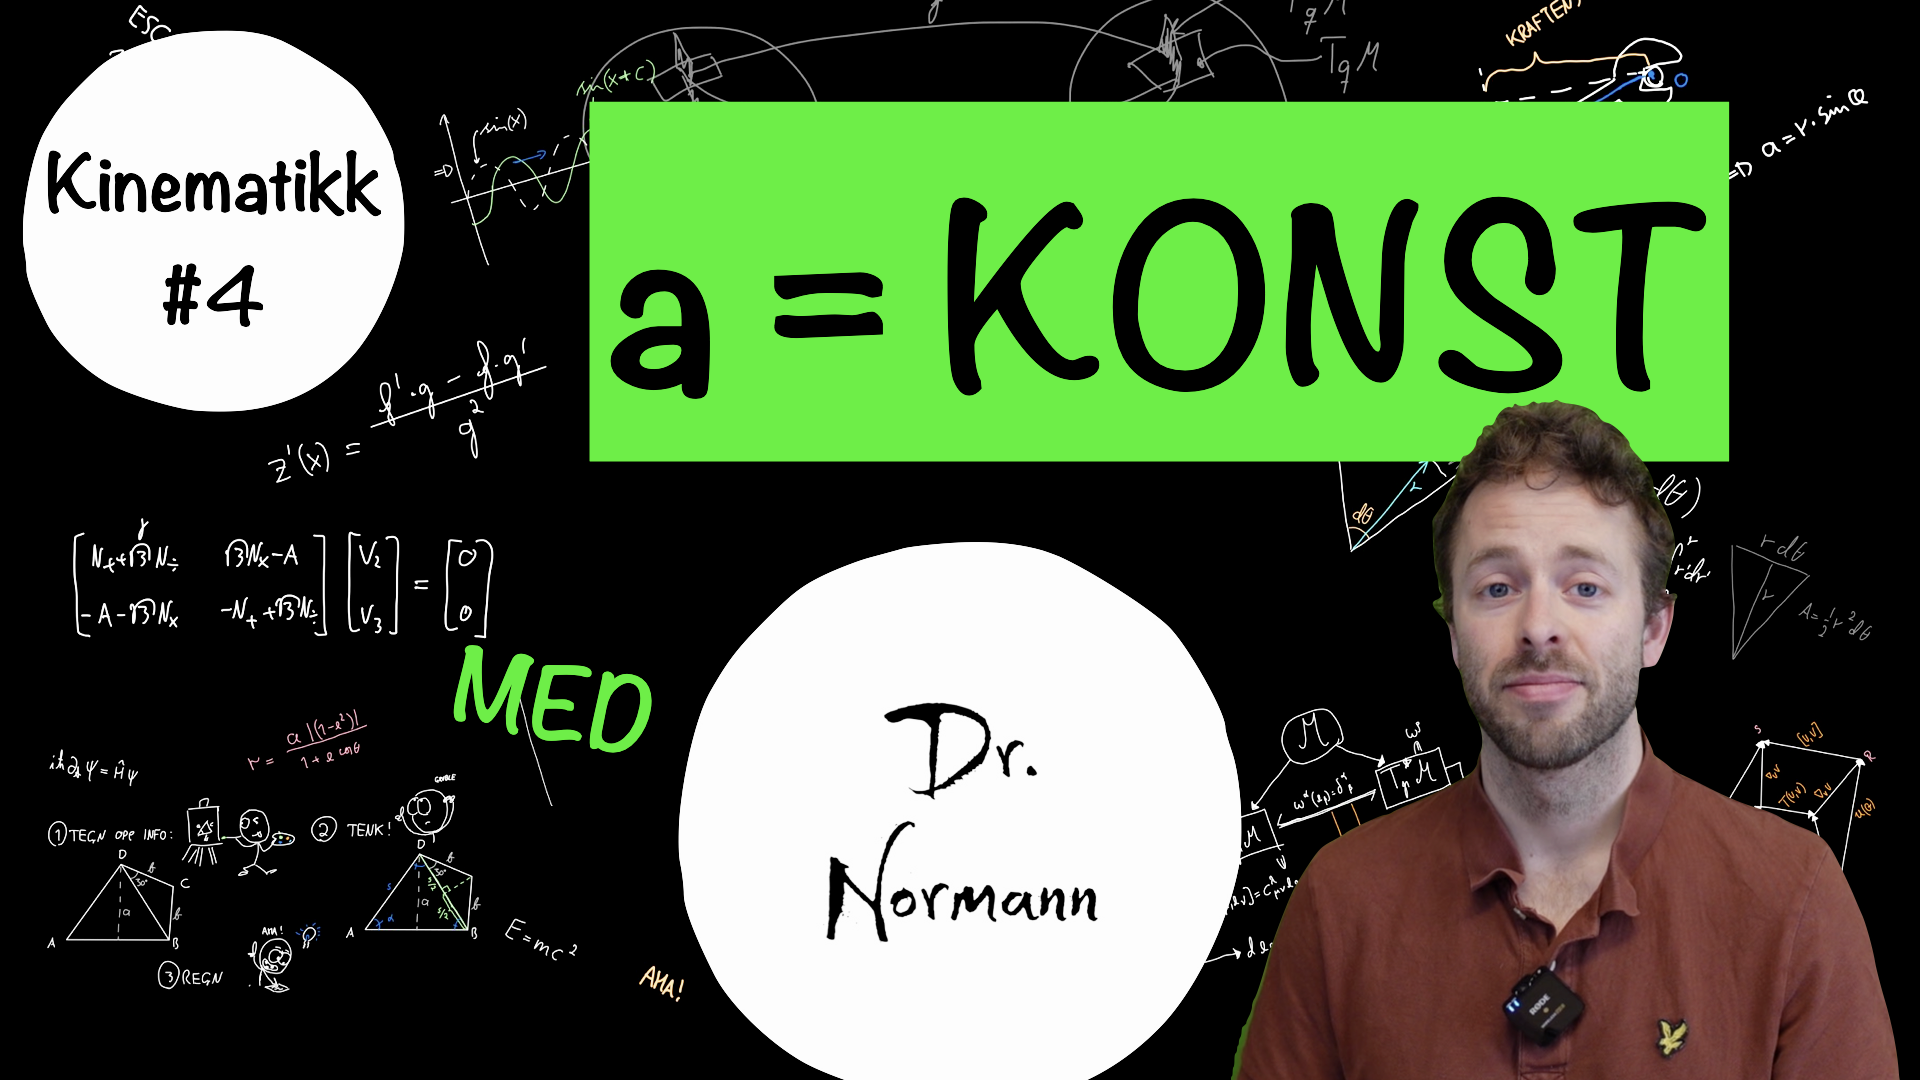
\includegraphics[width=3.6cm]{Images/YouTubeLenker/YT_KonstantAkselerasjon.png}};
\node[anchor=north west] at (thumb.south west) {
\includegraphics[width=1.2cm]{Images/YouTubeLenker/Icon.png}};
\end{tikzpicture}%
}}%
\end{wrapfigure}
Noen ganger er akselerasjonen konstant, $a = \mathrm{konst.}$ Dette er en god antakelse i mange situasjoner, slik som fritt fall eller jevn bremsing.Bevegelseslikningene kan da utledes geometrisk ved hjelp av \textit{arealet under grafen}: arealet under $a(t)$-grafen gir endring i fart, og arealet under $v(t)$-grafen gir forflytning.

%--- Figur: a(t)-rektangel og v(t)-trapes side om side --------------------
% Skala: x = 4 cm tilsvarer tid t  |  y skalert for tydlighet
\begin{center}
\begin{minipage}[b]{0.46\textwidth}
  \centering
  %-- a(t): konstant → rektangel --
  \begin{tikzpicture}[font=\small]
    % Fylt rektangel (areal = Δv)
    \fill[headCol!15](0,0) rectangle (4,1.5);
    % Akser
    \draw[->,thick](-0.3,0)--(5.0,0) node[right]{$t$};
    \draw[->,thick](0,-0.3)--(0,2.3) node[above]{$a(t)$};
    % Konstant akselerasjon
    \draw[headCol,thick](0,1.5)--(4,1.5);
    % Høyre kant (stengsel)
    \draw[gray!50,dashed,thin](4,0)--(4,1.5);
    % Strekmerker
    \draw[thin](4,2.5pt)--(4,-2.5pt);
    \node[below=3pt,font=\scriptsize]at(4,0){$t$};
    \draw[thin](-2.5pt,1.5)--(2.5pt,1.5);
    \node[left=4pt,font=\scriptsize]at(0,1.5){$a$};
    \node[below left=1pt,font=\scriptsize]at(0,0){$0$};
    % Arealmerking
    \node[font=\scriptsize]at(2,0.75){areal $= a\cdot t = \Delta v$};
    % Usynlig node: holder bredde lik høyre figur
    \node[right=2pt,opacity=0,font=\scriptsize]at(4.5,1.4){$s{-}s_0$};
  \end{tikzpicture}

  \smallskip
  {\footnotesize \textbf{(a)} $a(t)$-grafen. Arealet av rektangelet er endringen i fart: $\Delta v = v - v_0$.}
\end{minipage}\hfill
\begin{minipage}[b]{0.46\textwidth}
  \centering
  %-- v(t): stigende linje → trapes = rektangel + trekant --
  % v₀ = 1.0 cm, v = v₀+at = 2.8 cm, t = 4 cm
  \begin{tikzpicture}[font=\small]
    % Rektangel (v₀·t)
    \fill[headCol!15](0,0)--(4,0)--(4,1.0)--(0,1.0)--cycle;
    % Trekant (½at²)
    \fill[oppsumcol!20](0,1.0)--(4,1.0)--(4,2.8)--cycle;
    % Akser
    \draw[->,thick](-0.3,0)--(5.0,0) node[right]{$t$};
    \draw[->,thick](0,-0.3)--(0,3.5) node[above]{$v(t)$};
    % v(t)-linje
    \draw[headCol,thick](0,1.0)--(4,2.8);
    % Hjelpelinjer
    \draw[gray!50,dashed,thin](0,1.0)--(4,1.0);
    \draw[gray!50,dashed,thin](4,0)--(4,2.8);
    % Strekmerker
    \draw[thin](4,2.5pt)--(4,-2.5pt);
    \node[below=3pt,font=\scriptsize]at(4,0){$t$};
    \draw[thin](-2.5pt,1.0)--(2.5pt,1.0);
    \node[left=4pt,font=\scriptsize]at(0,1.0){$v_0$};
    \draw[thin](-2.5pt,2.8)--(2.5pt,2.8);
    \node[left=4pt,font=\scriptsize]at(0,2.8){$v$};
    \node[below left=1pt,font=\scriptsize]at(0,0){$0$};
    % Arealmerking
    \node[font=\scriptsize]at(2,0.46){$v_0\cdot t$};
    \node[font=\scriptsize]at(3.1,1.85){$\tfrac{1}{2}at^2$};
    % Dobbelpil: total Δs
    \draw[<->,thin,black!50](4.4,0)--(4.4,2.8);
    \node[right=2pt,font=\scriptsize]at(4.4,1.4){$s{-}s_0$};
  \end{tikzpicture}

  \smallskip
  {\footnotesize \textbf{(b)} $v(t)$-grafen. Trapesarealet (rektangel $+$ trekant) er forflytningen: $\Delta s = s - s_0$.}
\end{minipage}
\end{center}

\medskip

\paragraph{Likning 1 – Hastighetslikningen.}
Siden $a(t) = a$ er konstant, er akselerasjonsgrafen en horisontal linje (figur~(a)). Arealet av rektangelet under grafen er lik endringen i fart:
\[
  a \cdot t \;=\; \Delta v \;=\; v - v_0.
\]
Løser vi for $v$ får vi:
\begin{align}
  \colorbox{black!7}{$\displaystyle v = v_0 + at$}
\end{align}

\paragraph{Likning 2 – Posisjonslikningen.}
Fartsgrafen $v(t) = v_0 + at$ er en stigende rett linje (figur~(b)). Arealet under den – trapeset fra $0$ til $t$ – er forflytningen $\Delta s = s - s_0$. Vi deler trapeset i to deler: et rektangel med bredde $t$ og høyde $v_0$ (areal $= v_0\,t$), og en trekant med base $t$ og høyde $at$ (areal $= \tfrac{1}{2}at^2$). Totalt:
\[
  s - s_0 \;=\; v_0\,t + \tfrac{1}{2}at^2,
\]
altså:
\begin{align}
  \colorbox{black!7}{$\displaystyle s = s_0 + v_0\,t + \tfrac{1}{2}at^2$}
\end{align}

\paragraph{Likning 3 – Fart-strekning-likningen.}
Likning~3 følger algebraisk av likning~1 og~2. Fra likning~1 er $t = (v - v_0)/a$. Setter vi dette inn i likning~2:
\begin{align*}
  s - s_0
  &= v_0\cdot\frac{v-v_0}{a} + \tfrac{1}{2}a\left(\frac{v-v_0}{a}\right)^2
   = \frac{v_0(v-v_0)}{a} + \frac{(v-v_0)^2}{2a}
   = \frac{(v-v_0)\bigl(2v_0 + v - v_0\bigr)}{2a}
   = \frac{v^2 - v_0^2}{2a}.
\end{align*}
Multipliserer vi med $2a$:
\begin{align}
  \colorbox{black!7}{$\displaystyle 2a(s-s_0) = v^2 - v_0^2$}
\end{align}

\paragraph{Likning 4 – Gjennomsnittshastighetslikningen.}
Et trapes med parallelle sider $v_0$ og $v$ har gjennomsnittshøyde $(v_0 + v)/2$. Arealet (forflytningen) kan derfor skrives:
\begin{align}
  \colorbox{black!7}{$\displaystyle s - s_0 = \frac{v_0 + v}{2}\cdot t$}
\end{align}
Dette viser at gjennomsnittshastigheten ved konstant akselerasjon er gjennomsnittet av start- og sluttfarten: $\bar{v} = (v_0 + v)/2$.

Selv om vi nå har utledet formlene over ved hjelp av de skalare størrelsene, sp gjelder de samme relasjonene også for krumlinjet bevegelse, hvor vi altså må benytte vektorer. I oppsumeringen under har vi derfor skrevet likningene i vektorform, slik at de gjelder for alle typer bevegelse – både rettlinjet og krumlinjet.
\begin{myoppsum*}{Bevegelseslikningene ved konstant akselerasjon}
\paragraph{1. Hastighetslikningen} gir hastighetsvektoren som funksjon av tid:
    \begin{align}
        \vec{v} = \vec{v}_0 + \vec{a}\,t
    \end{align}

\paragraph{2. Posisjonslikningen} gir posisjonsvektoren som funksjon av tid:
    \begin{align}
        \vec{s} = \vec{s}_0 + \vec{v}_0\,t + \tfrac{1}{2}\vec{a}\,t^2
    \end{align}

\paragraph{3. Fart-strekning-likningen} kopler fart og posisjon uten tid:
    \begin{align}
       |\vec{v}|^2 = |\vec{v}_0|^2 + 2\,\vec{a} \cdot (\vec{s} - \vec{s}_0)
    \end{align}

\paragraph{4. Gjennomsnittshastighetslikningen} (gjelder kun ved konstant $\vec{a}$):
    \begin{align}
        \vec{s} - \vec{s}_0 = \frac{\vec{v}_0 + \vec{v}}{2}\,t, \qquad \bar{\vec{v}} = \frac{\vec{v}_0 + \vec{v}}{2}
    \end{align}
\end{myoppsum*}

I spesialtilfellet med rettlinjet bevegelse (bevegelse langs én akse) trenger vi selvsagt ikke vektortegnene, siden retningen uttrykkes fullt ut ved fortegnet til de skalare størrelsene. Da er det de opprinnelige, skalare likningene --- slik vi utledet dem tidligere i dette avsnittet --- som gjelder.

Vi setter dessuten ofte $s_0 = 0$ i praksis, ettersom $s_0$ bare er startposisjonen --- og vi kan alltid velge koordinatsystemet slik at bevegelsen starter i origo.

\tips{Alternativ utledning med integrasjon}{%
Likning 1 og 2 kan også utledes ved integrasjon. Siden $a$ er konstant, integrerer vi over tid:
\[
  v(t) = \int a\,\mathrm{d}t = at + v_0,
\]
der $v_0$ er integrasjonskonstanten, som vi tolker som startfarten (farten ved $t=0$). Integrerer vi én gang til:
\[
  s(t) = \int v\,\mathrm{d}t = \int(v_0 + at)\,\mathrm{d}t = v_0\,t + \tfrac{1}{2}at^2 + s_0,
\]
der $s_0$ er startposisjonen. Likning 3 og 4 følger deretter algebraisk, som vist i utledningen ovenfor.
}

 Disse fire likningene gir et komplett sett med verktøy for å analysere bevegelse under konstant akselerasjon. Det er imidlertid avgjørende å huske at de bare gjelder når akselerasjonen ikke varierer. Hvis akselerasjonen endrer seg, blir bevegelsen mer kompleks, og disse likningene vil ikke lenger være gyldige.

\exm{Bremseavstand}{
En bil har en startfart på \(30 \, \si{\metre\per\second}\) og bremser med en konstant akselerasjon på \(-5 \, \si{\metre\per\second\squared}\). Hvor langt beveger bilen seg før den stopper helt? \\

\textit{Metode:}
Bruk hastighet-posisjonslikningen \( v^2 = v_0^2 + 2a(s - s_0) \). Her er \( v = 0 \, \si{\metre\per\second} \), \( v_0 = 30 \, \si{\metre\per\second} \), og \( a = -5 \, \si{\metre\per\second\squared} \):
\[
0 = (30 \, \si{\metre\per\second})^2 + 2 \cdot (-5 \, \si{\metre\per\second\squared}) \cdot (s - s_0).
\]
\[
0 = \SI{900}{\metre\squared\per\second\squared} - \SI{10}{\metre\per\second\squared} \cdot (s - s_0).
\]
\[
\SI{10}{\metre\per\second\squared} \cdot (s - s_0) = \SI{900}{\metre\squared\per\second\squared}
\]
\[
s - s_0 = \doubleunderline{90 \, \si{\metre}}
\]
Bilen beveger seg $\SI{90}{\metre}$ før den stopper.
}

\exm{Sykkeltur}{
Du sykler med en startfart på \(5 \, \si{\metre\per\second}\) og akselererer til \(15 \, \si{\metre\per\second}\) over en tidsperiode på \(10\) sekunder. Hvor langt syklet du i denne perioden? \\

\textit{Metode:}
Bruk gjennomsnittshastighetslikningen \( s = s_0 + \frac{v_0 + v}{2}t \). Her er \( s_0 = 0 \, \si{\metre} \), \( v_0 = 5 \, \si{\metre\per\second} \), \( v = 15 \, \si{\metre\per\second} \), og \( t = 10 \, \si{\second} \):
\[
s = \SI{0}{\metre} + \frac{\SI{5}{\metre\per\second} + \SI{15}{\metre\per\second}}{2} \cdot \SI{10}{\second} = \doubleunderline{100 \, \si{\metre}}
\]
Du syklet $\SI{100}{\metre}$ i løpet av denne perioden.
}



\subsection{Fritt fall som eksempel}
Her på jorden blir vi påvirket av en tyngdekraft, som gjør at alt blir dratt mot senter av jorden. Det som kanskje er litt overraskende, er at alle legemer vil ha samme akselerasjon ned mot bakken (når vi ser bort ifra luftmotstand). Denne akselerasjonen er konstant og kalles $\text{g}$. Størrelsen er
\graabox{$\displaystyle \text{Tyngdens akselerasjon:}\quad\text{g} = \SI{9.81}{\metre\per\second\squared}$}

Legemer som kun er under påvirkning av tyngdekraften, sies å være i \textbf{fritt fall}. En bergknaus som faller fra fjellet og nedover mot fjorden er for eksempel i fritt fall. Eller — ikke helt; vi må jo huske luftmotstanden, som også påvirker knausens bevegelse gjennom lufta. Noen ganger simulerer man vektløshet i fly. Dette er å simulere fritt fall. Inne i flyet så fallre jo lufta sammen med deg, og du påvirkes derfor ikke av luftmotstand heller. Dermed får man til fritt fall, som altså er det samme som vektløshet. Hadde du tatt med en baderomsvekt opp i flyet, ville du sett at vekten viste 0 kg under fritt fall! Fin (men kortvarig) jubel over vektnedgang ;)

\tanke{}{
Dersom alle legemer faller med lik akselerasjon under fritt fall, hvorfor faller da et papirark saktere enn en stein mot bakken?
}

\exm{Hastighetsendring}{
Tenk deg at du kaster en ball rett opp i luften med en startfart på \(10 \, \si{\metre\per\second}\). Tyngdekraften gir ballen en konstant akselerasjon på \(-9.81 \, \si{\metre\per\second\squared}\). Hvor raskt beveger ballen seg etter \(2\) sekunder? \\

\textit{Metode:}
Bruk hastighetslikningen \( v = v_0 + at \). Her er \( v_0 = 10 \, \si{\metre\per\second} \), \( a = -9.81 \, \si{\metre\per\second\squared} \), og \( t = 2 \, \si{\second} \). Sett inn verdiene:
\[
v = 10 \, \si{\metre\per\second} + (-9.81 \, \si{\metre\per\second\squared}) \cdot 2 \, \si{\second} = \doubleunderline{-9.62 \, \si{\metre\per\second}}
\]
Ballens hastighet etter $2$ sekunder er $\SI{-9.62}{\metre\per\second}$, noe som indikerer at ballen nå beveger seg nedover.
}

\exm{Fallende objekt}{
En stein blir sluppet fra en bro \(20 \, \si{\metre}\) over bakken. Hva er steinens posisjon etter \(2\) sekunder, gitt at akselerasjonen på grunn av tyngdekraften er \(9.81 \, \si{\metre\per\second\squared}\) og initial hastighet \( v_0 = 0 \)? \\

\textit{Metode:}
Bruk posisjonslikningen \( s = s_0 + v_0t + \frac{1}{2}at^2 \). Her er \( s_0 = 20 \, \si{\metre} \), \( v_0 = 0 \, \si{\metre\per\second} \), \( a = 9.81 \, \si{\metre\per\second\squared} \), og \( t = 2 \, \si{\second} \):
\[
s = 20 \, \si{\metre} + \SI{0}{\metre\per\second} \cdot 2 \, \si{\second} + \frac{1}{2} \cdot 9.81 \, \si{\metre\per\second\squared} \cdot (2 \, \si{\second})^2
  = \SI{20}{\metre} + \SI{19.62}{\metre}.
\]
\[
s = \doubleunderline{39.6 \, \si{\metre}}
\]
Steinen er $\SI{39.6}{\metre}$ fra utgangspunktet etter $2$ sekunder.
}


\oppgave{Sten i fritt fall}{%
\begin{enumerate}[a)]
    \item En sten faller utfor preikestolen. Hva er akselerasjonen til steinen (se bort ifra luftmotstand)
    \item En sten kastes rett oppover, og faller rett ned igjen. Hva er akselerasjonen til steinen (i) på vei opp, (ii) på toppen og (ii) på vei ned? Tegn figur og forklar kort med ord. 
\end{enumerate}
}

\oppgave{Fritt fall}{%
En ball slippes fra ro fra en høyde $h = \SI{45}{\metre}$ over bakken. Husk at $\text{g} = \SI{9.81}{\metre\per\second\squared}$.
\begin{enumerate}[a)]
    \item Finn tiden det tar før ballen treffer bakken.
    \item Finn farten rett før ballen treffer bakken.
    \item Hva ville farten blitt om ballen var sluppet fra $h = \SI{80}{\metre}$? Legg merke til sammenhengen.
\end{enumerate}
}

\subsection{Dekomponering ved krumlinjet bevegelse}
Vi har tidligere utledet formler for 
$$a=\text{konst},$$
og brukt vektorer i oppsummeringen, fordi disse formlene gjelder for krumlinjet bevegelse også. Men hvordan regner vi egentlig med konstant akselerasjon i krumlinjet bevegelse i praksis? I denne seksjonen skal vi se på nettopp det, gjennom eksempler og oppgaver.

\paragraph{Dekomponering.} Se for deg en stein som kastes utfor en klippe. Steinen vil falle nedover på grunn av tyngdekraftens konstante akselerasjon på $\text{g}=\SI{9.81}{\metre\per\second\squared}$. Men i horisontal retning så vil steinen bare fortsette rett fram uten å akselerere. Vi må \textit{dekomponere} likningene og analysere hver retning for seg. 

\begin{myoppsum*}{Dekomponering av hastighets- og posisjonslikningene}
Krumlinjet bevegelse med konstant akselerasjon analyseres ved å dekomponere vektorlikningene i x- og y-komponenter:

\medskip
\textbf{Hastighetslikningen:}
\[
  \vec{v} = \vec{v}_0 + \vec{a}\,t
  \quad\Longrightarrow\quad
  \begin{cases}
    v_x = v_{0x} + a_x\,t \\[5pt]
    v_y = v_{0y} + a_y\,t
  \end{cases}
\]

\medskip
\textbf{Posisjonslikningen:}
\[
  \vec{s} = \vec{s}_0 + \vec{v}_0\,t + \tfrac{1}{2}\vec{a}\,t^2
  \quad\Longrightarrow\quad
  \begin{cases}
    x = x_0 + v_{0x}\,t + \tfrac{1}{2}a_x\,t^2 \\[5pt]
    y = y_0 + v_{0y}\,t + \tfrac{1}{2}a_y\,t^2
  \end{cases}
\]
\end{myoppsum*}
Vi kunne gjort tilsvarende dekomponeringer av de to andre likningene — og hvilke som helst andre vektorlikninger.

\tips{Fortegn ved dekomponering}{Husk at når du dekomponerer så er alle fortegn avhengig av hva du har valt som positiv retning for hver koordinat-akse. For eksempel, hvis du velger oppover som positiv y-retning, så vil tyngdekraftens akselerasjon i y-retning være negativ, altså $a_y = -g$. Hvis du velger nedover som positiv y-retning, så vil tyngdekraftens akselerasjon i y-retning være positiv, altså $a_y = g$. Dette er bare et valg av koordinatsystem, og har ingen innvirkning på fysikken.
}
La oss nå se på eksempler for å lære dette med dekomponering ordentlig.

\exm{Straffespark}{
Håland skal skyte et straffespark, og skyter ballen med en utgangsvinkel på $18^\circ$ i forhold til bakken, se figur~\ref{fig:straffespark}. Straffemerket ligger $\SI{11}{\metre}$ fra mållinjen. Et fotballmål er internasjonalt standardisert til å være $\SI{2.44}{\metre}$ høyt (avstanden fra bakken til undersiden av tverrliggeren). Ballen har imidlertid selv en viss utstrekning, så det holder at \textit{senteret} av ballen befinner seg i høyden $\SI{2.30}{\metre}$ for at ballen så vidt skal passere under tverrliggeren. Håland ønsker å skyte ballen slik at den passerer rett under tverrliggeren, akkurat idet den når mållinjen. Vi ser bort fra luftmotstand. Hvor stor må utgangsfarten $v_0$ være?\\

    \textbf{Del a: Sett opp posisjonslikningene} \\

    \textit{Metode:}
    Vi lar $x$ være den horisontale avstanden fra straffemerket, og $y$ være høyden over bakken. Startposisjonen er $x_0 = 0$ og $y_0 = 0$, og komponentene av utgangsfarten er $v_{0x} = v_0\cos\theta$ og $v_{0y} = v_0\sin\theta$, hvor $\theta = 18^\circ$. Det er ingen akselerasjon i $x$-retning, mens akselerasjonen i $y$-retning er tyngdeakselerasjonen $a_y = -g$. Posisjonslikningene blir dermed:
    \[
    x(t) = v_0 \cos\theta \cdot t, \qquad y(t) = v_0 \sin\theta \cdot t - \frac{1}{2} g t^2.
    \]

    \textbf{Del b: Finn tiden $t^\ast$ ballen bruker til mållinjen} \\

    \textit{Metode:}
    Ballen når mållinjen når $x(t^\ast) = \SI{11}{\metre}$. Fra uttrykket for $x(t)$ i Del a løser vi for $t^\ast$:
    \[
    t^\ast = \frac{11}{v_0 \cos\theta}.
    \]

    \textbf{Del c: Finn utgangsfarten $v_0$} \\

    \textit{Metode:}
    Idet ballen når mållinjen skal ballens senter befinne seg i høyden $y(t^\ast) = \SI{2.30}{\metre}$ (rett under tverrliggeren, når vi tar hensyn til ballens egen utstrekning). Vi setter $t^\ast$ fra Del b inn i uttrykket for $y(t)$:
    \[
    2.30 = v_0 \sin\theta \cdot \frac{11}{v_0 \cos\theta} - \frac{1}{2} g \left( \frac{11}{v_0 \cos\theta} \right)^2 = 11 \tan\theta - \frac{121\, g}{2 v_0^2 \cos^2\theta}.
    \]
    Legg merke til at $v_0$ forsvinner fra det første leddet, siden $\sin\theta / \cos\theta = \tan\theta$. Vi løser likningen for $v_0^2$:
    \[
    v_0^2 = \frac{121\, g}{2\cos^2\theta \left( 11\tan\theta - 2.30 \right)}.
    \]
    Setter vi inn tallverdiene $g = \SI{9.81}{\metre\per\second\squared}$ og $\theta = 18^\circ$, får vi
    \[
    v_0 = \doubleunderline{\SI{22.7}{\metre\per\second}} \approx \SI{81.7}{\kilo\metre\per\hour}.
    \]
    Dette er en realistisk fart for et hardt skutt straffespark.
}

   \begin{figure}[ht!]
    \centering
    \usetikzlibrary{calc}
    \begin{tikzpicture}
    \node[anchor=south west, inner sep=0pt] (img) at (0,0) {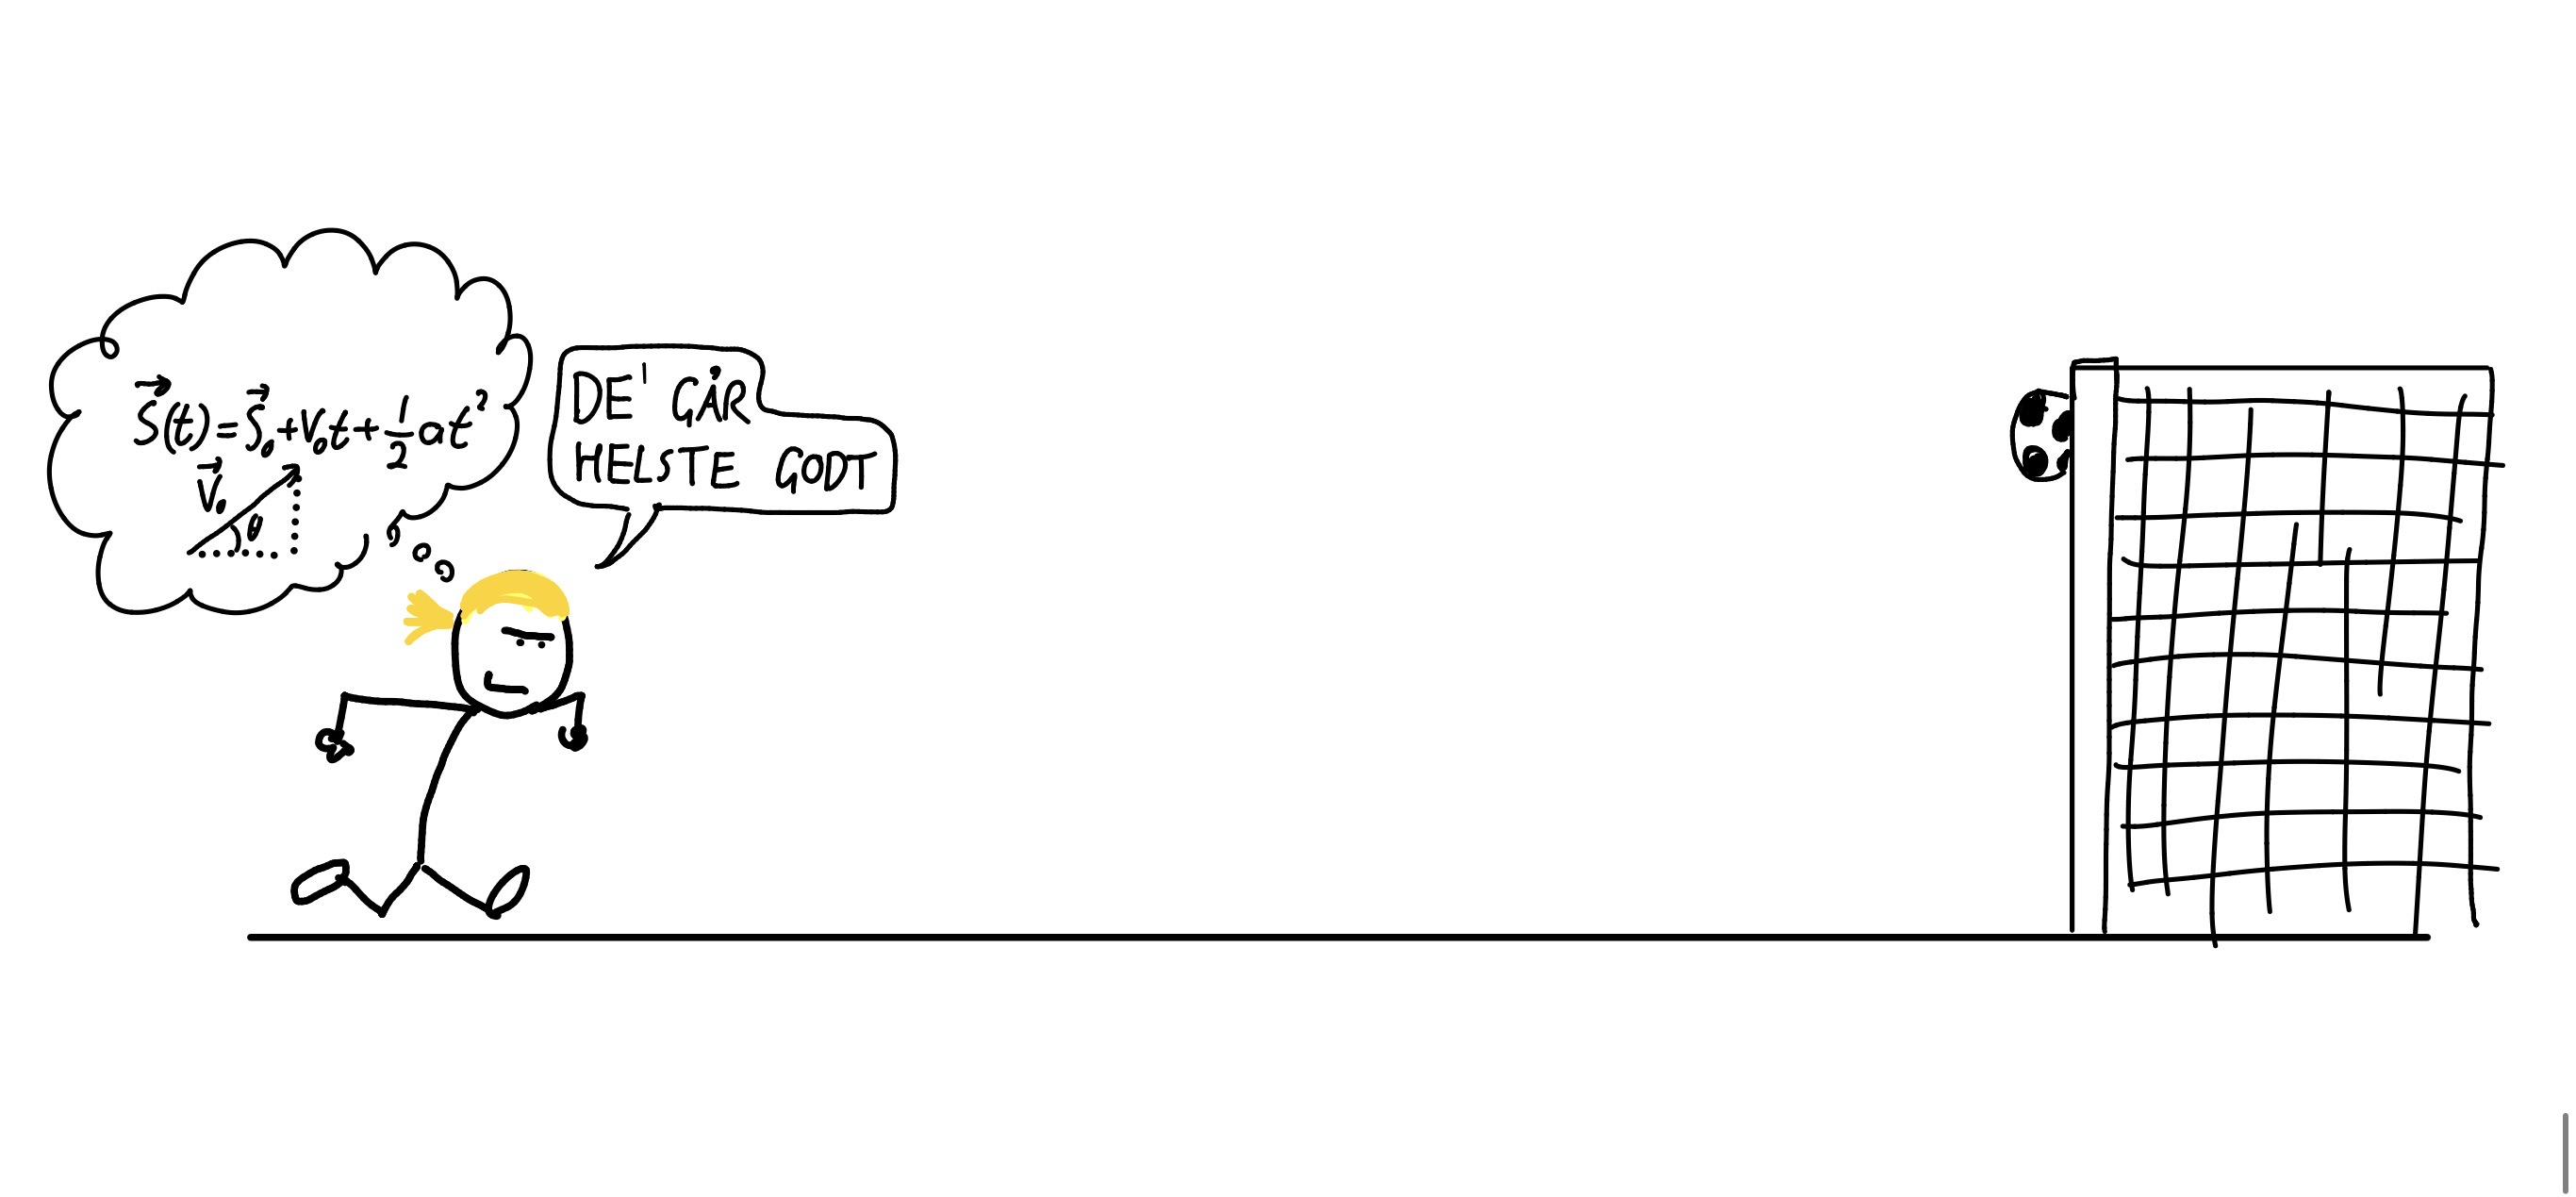
\includegraphics[width=0.8\textwidth]{Images/Kapittel2:Kinematikk/Straffespark_Haaland.png}};
    \newcommand{\imgpt}[3]{%
        \coordinate (#1tmpx) at ($(img.south west)!#2!(img.south east)$);%
        \coordinate (#1tmpy) at ($(img.south west)!#3!(img.north west)$);%
        \coordinate (#1) at (#1tmpx |- #1tmpy);%
    }
    \imgpt{Foot}{0.213}{0.278}
    \imgpt{Ball}{0.757}{0.653}
    \imgpt{FootGround}{0.213}{0.2175}
    \imgpt{PostGround}{0.798}{0.2175}
    \imgpt{Hleft}{0.213}{0.16}
    \imgpt{Hright}{0.798}{0.16}
    \imgpt{Vbottom}{0.68}{0.2175}
    \imgpt{Vtop}{0.68}{0.653}
    \imgpt{Hlabel}{0.5055}{0.13}
    \imgpt{Vlabel}{0.625}{0.435}
    % Punkter langs parabelbanen (kun krumning mot horisontal, tangent til v0 i Foot)
    \imgpt{Traj0}{0.2130}{0.2780}
    \imgpt{Traj1}{0.2493}{0.3408}
    \imgpt{Traj2}{0.2855}{0.3982}
    \imgpt{Traj3}{0.3218}{0.4502}
    \imgpt{Traj4}{0.3581}{0.4968}
    \imgpt{Traj5}{0.3943}{0.5380}
    \imgpt{Traj6}{0.4306}{0.5739}
    \imgpt{Traj7}{0.4669}{0.6043}
    \imgpt{Traj8}{0.5031}{0.6293}
    \imgpt{Traj9}{0.5394}{0.6489}
    \imgpt{Traj10}{0.5757}{0.6630}
    \imgpt{Traj11}{0.6119}{0.6718}
    \imgpt{Traj12}{0.6482}{0.6752}
    \imgpt{Traj13}{0.6845}{0.6732}
    \imgpt{Traj14}{0.7207}{0.6658}
    % Parabelbane fra Hålands fot til ballen
    \draw[dashed, very thick, exmscol]
      (Traj0) -- (Traj1) -- (Traj2) -- (Traj3) -- (Traj4) -- (Traj5) -- (Traj6) -- (Traj7)
      -- (Traj8) -- (Traj9) -- (Traj10) -- (Traj11) -- (Traj12) -- (Traj13) -- (Traj14) -- (Ball);
    % Fartsvektoren v0, tangent til banen ved avspark
    \draw[dotted, black!50] (Foot) -- ($(Foot)+(1.6,0)$);
    \draw[->, very thick, exmscol] (Foot) -- ++(40:1.6) node[above right=1pt, exmscol] {\large $\vec{v}_0$};
    \draw[black!60] ($(Foot)+(0.7,0)$) arc (0:40:0.7);
    \node[font=\small, black!60] at ($(Foot)+({0.95*cos(20)},{0.95*sin(20)})$) {$\theta$};
    % 11 m -- horisontal avstand fra Håland til stolpen
    \draw[<->, thick, mycolor] (Hleft) -- (Hright);
    \draw[dotted, mycolor!50] (FootGround) -- (Hleft);
    \draw[dotted, mycolor!50] (PostGround) -- (Hright);
    \node[below=2pt, mycolor] at (Hlabel) {\large $11\,\text{m}$};
    % 2.30 m -- vertikal høyde fra bakken opp til ballen, plassert utenfor målet
    \draw[<->, thick, mycolor] (Vbottom) -- (Vtop);
    \draw[dotted, mycolor!50] (Vtop) -- (Ball);
    \node[left=2pt, mycolor] at (Vlabel) {\large $2.30\,\text{m}$};
    \end{tikzpicture}
    \caption{Straffespark. Ballens bane er vist med stiplet linje, med utgangsfarten $\vec{v}_0$ tegnet inn som tangent til banen ved avspark.}
    \label{fig:straffespark}
    \end{figure}

\exm{Rallybil kjører utfor}{
En rallybil kjører utfor banen. Den starter med farten $v_0 = \SI{80}{\kilo\metre\per\hour}$. Fordi den kjører over et jorde og gjennom noen busker, bremses farten, slik at den til slutt er $v_1 = \SI{30}{\kilo\metre\per\hour}$. Vi antar at denne oppbremsingen skjer med konstant akselerasjon over en strekning på $\SI{50}{\metre}$. Deretter kjører bilen utfor en klippe og lander $\SI{5}{\metre}$ lenger nede, se figur~\ref{fig:rallybil}.
\begin{itemize}
    \item a) Bestem akselerasjonen på strekningen.
    \item b) Finn ut hvor langt bort den beveger seg i horisontal retning før den treffer bakken.
    \item c) Finn fartsvektoren i det bilen treffer bakken.
\end{itemize}

    \textbf{Del a: Beregn akselerasjonen} \\

    \textit{Metode:}
    Vi regner om fartene til SI-enheter:
    \[
    v_0 = \SI{80}{\kilo\metre\per\hour} = \SI{22.2}{\metre\per\second}, \qquad v_1 = \SI{30}{\kilo\metre\per\hour} = \SI{8.33}{\metre\per\second}.
    \]
    Siden akselerasjonen er konstant, og vi kjenner start- og sluttfart samt strekningen $\Delta s = \SI{50}{\metre}$, bruker vi likningen $v_1^2 = v_0^2 + 2a\,\Delta s$. Vi løser for $a$:
    \[
    a = \frac{v_1^2 - v_0^2}{2\,\Delta s} = \frac{(8.33)^2 - (22.2)^2}{2\cdot 50} \approx \doubleunderline{-4.24 \, \si{\metre\per\second\squared}}.
    \]
    Akselerasjonen er negativ, altså en oppbremsing (retardasjon), som vi forventer.

    \textbf{Del b: Finn horisontal avstand $x$} \\

    \textit{Metode:}
    Idet bilen kjører utfor klippen har den kun horisontal fart, $v_{0x} = v_1 = \SI{8.33}{\metre\per\second}$, og ingen vertikal fart, $v_{0y} = 0$. Vi lar $y_0 = \SI{5}{\metre}$ være klippens høyde, med $y = 0$ ved bakken. Posisjonslikningen i $y$-retning gir tiden $t$ bilen er i lufta:
    \[
    y = y_0 + v_{0y} t - \frac{1}{2} g t^2 \quad \Rightarrow \quad 0 = 5 - \frac{1}{2}(9.81) t^2 \quad \Rightarrow \quad t = \sqrt{\frac{2\cdot 5}{9.81}} \approx \SI{1.01}{\second}.
    \]
    Horisontal avstand følger av $x = v_{0x} t$ (ingen akselerasjon i $x$-retning):
    \[
    x = 8.33 \cdot 1.01 \approx \doubleunderline{\SI{8.41}{\metre}}.
    \]

    \textbf{Del c: Finn fartsvektoren idet bilen treffer bakken} \\

    \textit{Metode:}
    Den horisontale hastighetskomponenten er uendret, $v_x = v_{0x} = \SI{8.33}{\metre\per\second}$. Den vertikale komponenten finner vi fra hastighetslikningen:
    \[
    v_y = v_{0y} - g t = 0 - 9.81 \cdot 1.01 \approx \SI{-9.90}{\metre\per\second}.
    \]
    Fartsvektoren er dermed $\vec{v} = [\SI{8.33}{\metre\per\second},\, \SI{-9.90}{\metre\per\second}]$, med størrelse
    \[
    v = \sqrt{v_x^2 + v_y^2} = \sqrt{8.33^2 + 9.90^2} \approx \doubleunderline{\SI{12.9}{\metre\per\second}},
    \]
    og retning
    \[
    \theta = \arctan\left(\frac{|v_y|}{v_x}\right) = \arctan\left(\frac{9.90}{8.33}\right) \approx \doubleunderline{50^\circ} \text{ under horisontalen}.
    \]
}

   \begin{figure}[ht!]
    \centering
    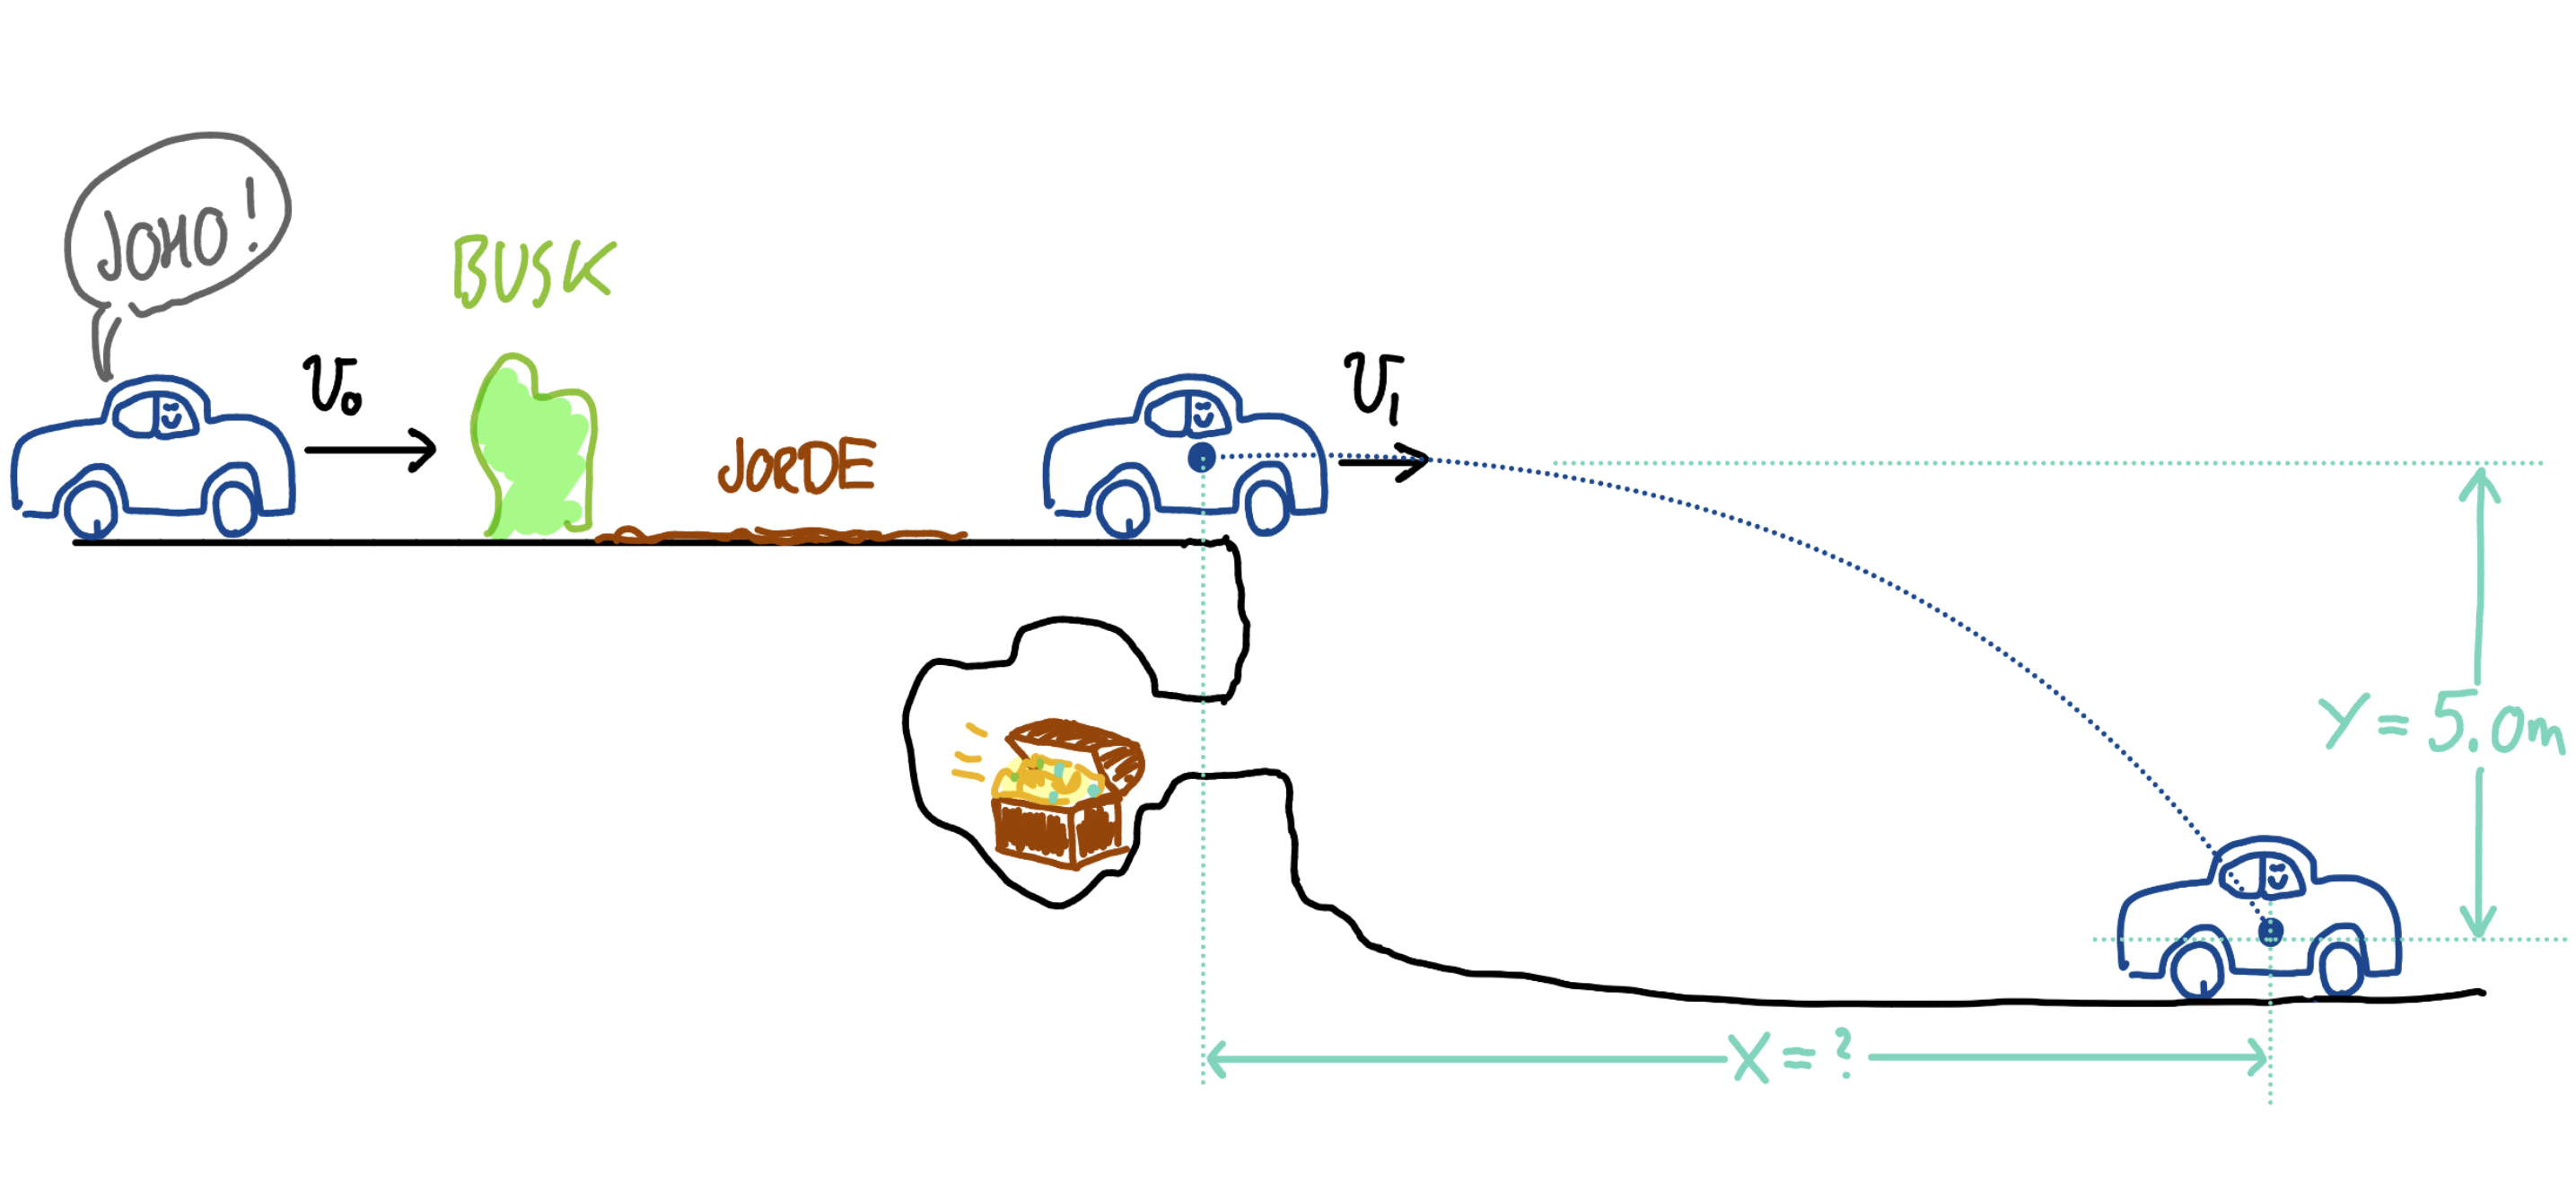
\includegraphics[width=0.8\textwidth]{Images/Kapittel2:Kinematikk/RallybilKlippe.png}
    \caption{Rallybilen kjører utfor klippen}
    \label{fig:rallybil}
\end{figure}

\oppgave{Ballkast}{%
En ball kastes horisontalt fra en klippe $h = \SI{5}{\metre}$ over bakken med startfart $v_0 = \SI{10}{\metre\per\second}$. Bruk $g = \SI{9.81}{\metre\per\second\squared}$.
\begin{enumerate}[a)]
    \item Finn tiden ballen bruker på å treffe bakken.
    \item Finn den horisontale avstanden fra klippen til der ballen lander.
    \item Finn farten (størrelsen av hastighetsvektoren) rett før ballen treffer bakken.
\end{enumerate}
}

\oppgave{Prosjektilbevegelse}{%
Et prosjektil skytes ut fra bakken ($y_0 = 0$) med en kjent utgangshastighet $v_0$, i en vinkel $\theta$ over horisontalen. Se bort fra luftmotstand.
\begin{enumerate}[a)]
    \item Sett opp uttrykk for posisjonen til prosjektilet i $x$- og $y$-retning som funksjon av tiden $t$.
    \item Finn et uttrykk for tiden $t$ prosjektilet er i lufta, uttrykt ved $v_0$, $\theta$ og $g$.

    \textit{Hint:} Bruk at prosjektilet returnerer til utgangshøyden når det lander, altså $y(t) = 0$.

    \item Bruk uttrykket for $t$ fra forrige punkt til å finne et uttrykk for hvor langt prosjektilet lander fra utgangspunktet (sluttposisjonen i $x$-retning).
    \item Skriv sluttposisjonen som en vektor $[x,\,y]$.
\end{enumerate}
}

\newpage

\section{Sirkelbevegelse}

\textit{Sirkelbevegelse} Vi Sirkelbevegelse er en form for krumlinjet bevegelse i planet som vi skal se ekstra nøye på. 
\tanke{}{%
I hvilken retning peker akselerasjonen i sirkelbevegelse?}

Se for deg at du sitter i en bil som holder konstant høy fart gjennom en rundkjøring. Du vil oppleve at du presses ut mo høyre i bilen (gitt at bilens kjøreretning er overholder norske trafikkregler!). Men om vi zoomer ut av bilen og tar perspektivet til den forskrekkede måken som sitter på en flaggstand midt i rundkjøringen, så ser vi tydelig at det ikke er det som skjer. Det som egentlig skjer er at bilen stadig endrer kjøreretning. Dette fører til at du (som passasjer i bilen) stadig aksellereres inn mot sentrum! Denne akselerasjonen kalles \textit{sentripetalakselerasjon}, og er altså grunnen til at det føles som om noe dytter deg ut av rundkjøringen, selv om det altså ikke er det som skjer.

\paragraph{Utledning av sentripetalakselerasjon} I det følgende skal vi utlede et uttrykk for størrelsen på sentripetalakselerasjon. 
Se for deg et legeme (f.eks. en bil) som holder konstant fart i sirkelbevegelse. Selv om farten \( v \) forblir konstant så endrer harstighetsvektoren \( \vec{v} \) seg, ettersom retningen til farten endres. Ser vi på to tidspunkt hvor hastigheten endrer seg fra \( \vec{v}_1 \) til \( \vec{v}_2 \), kan vi bruke forholdet mellom de formlike trekantene for \( \Delta \vec{v} \) og \( \Delta \vec{s} \), som gir oss:
    \[
    \frac{\Delta v}{v} = \frac{\Delta s}{r}.
    \]
    Der \( r \) er radiusen til sirkelen, og \( \Delta s \) er avstanden objektet har beveget seg langs sirkelen i løpet av et lite tidsintervall \( \Delta t \). 


\begin{figure}[h]
\centering
% LEFT: position diagram
\begin{minipage}[t]{0.50\textwidth}
\centering
\begin{tikzpicture}[font=\small, scale=1.15, >=stealth]
  % Centre O
  \fill (0,0) circle (2pt);
  \node[below left=2pt] at (0,0) {$O$};

  % Partial circle arc (40° – 140°)
  \draw[headCol, thick]
    ({2*cos(40)},{2*sin(40)}) arc[start angle=40, end angle=140, radius=2];

  % Points P1 (110°) and P2 (70°)
  \coordinate (P1) at ({2*cos(110)},{2*sin(110)});
  \coordinate (P2) at ({2*cos(70)},{2*sin(70)});

  % Radii
  \draw[black!40, semithick] (0,0) -- (P1);
  \draw[black!40, semithick] (0,0) -- (P2);

  % r labels at midpoints of radii
  \node[left=2pt,  black!55, font=\footnotesize] at ({cos(110)},{sin(110)}) {$r$};
  \node[right=2pt, black!55, font=\footnotesize] at ({cos(70)}, {sin(70)})  {$r$};

  % Angle Δθ arc at O
  \draw ({0.52*cos(110)},{0.52*sin(110)})
        arc[start angle=110, end angle=70, radius=0.52];
  \node[above=1pt, font=\footnotesize] at (0, 0.62) {$\Delta\theta$};

  % Points
  \fill[defscol] (P1) circle (2.5pt);
  \node[defscol, above left=2pt] at (P1) {$P_1$};
  \fill[defscol] (P2) circle (2.5pt);
  \node[defscol, above right=2pt] at (P2) {$P_2$};

  % Chord Δs (P1 → P2, horizontal since symmetric about 90°)
  \draw[->, oppsumcol, thick, dashed] (P1) -- (P2)
        node[midway, below=5pt] {$\Delta s$};

  % Velocity v1 at P1 (tangent = 110° − 90° = 20°)
  \draw[->, very thick, defscol]
        (P1) -- ++({cos(20)},{sin(20)})
        node[above right=-1pt] {$\vec{v}_1$};

  % Velocity v2 at P2 (tangent = 70° − 90° = −20°)
  \draw[->, very thick, defscol]
        (P2) -- ++({cos(-20)},{sin(-20)})
        node[right=2pt] {$\vec{v}_2$};
\end{tikzpicture}
\end{minipage}%
\hfill
% RIGHT: velocity triangle
\begin{minipage}[t]{0.46\textwidth}
\centering
\begin{tikzpicture}[font=\small, scale=1.15, >=stealth]
  % Tails at origin, v_len = 1.5
  \coordinate (tail) at (0,0);
  \coordinate (tip1) at ({1.5*cos(20)}, { 1.5*sin(20)});
  \coordinate (tip2) at ({1.5*cos(20)}, {-1.5*sin(20)});

  % v1 and v2
  \draw[->, very thick, defscol] (tail) -- (tip1);
  \draw[->, very thick, defscol] (tail) -- (tip2);

  % v labels along the arrows
  \node[defscol, above left=1pt, font=\footnotesize]
        at ({0.75*cos(20)},{ 0.75*sin(20)}) {$v$};
  \node[defscol, below left=1pt, font=\footnotesize]
        at ({0.75*cos(20)},{-0.75*sin(20)}) {$v$};

  % Arrow-head labels (v1, v2)
  \node[defscol, above=2pt]  at (tip1) {$\vec{v}_1$};
  \node[defscol, below=2pt]  at (tip2) {$\vec{v}_2$};

  % Δv from tip1 to tip2 (straight down)
  \draw[->, very thick, oppsumcol] (tip1) -- (tip2)
        node[right=3pt, midway] {$\Delta\vec{v}$};

  % Tail point
  \fill (tail) circle (1.5pt);

  % Angle Δθ at tail
  \draw ({0.52*cos(20)},{0.52*sin(20)})
        arc[start angle=20, end angle=-20, radius=0.52];
  \node[right=3pt, font=\footnotesize] at (0.60, 0) {$\Delta\theta$};

  % Bounding-box adjustment (match height of left panel)
  \path (0,0); \node[opacity=0] at (0,2.5) {$x$};
  \path (0,-1.7);
\end{tikzpicture}
\end{minipage}
\caption{Utledning av sentripetalakselerasjon.
\textbf{Venstre:} To nærliggende posisjoner $P_1$ og $P_2$ på sirkelbanen adskilt med vinkelen $\Delta\theta$. Hastighetsvektorene $\vec{v}_1$ og $\vec{v}_2$ er tangenter til banen.
\textbf{Høyre:} Hastighetstrekanten (vektorene lagt hale mot hale). De to trekantene er formlike med samme toppvinkel $\Delta\theta$ og forholdssidene $r$ og $v$, slik at $\Delta v/v = \Delta s/r$.}
\label{fig:Sentripetalakselerasjon}
\end{figure}
Formlikheten mellom trekantene er altså illustrert i figur~\ref{fig:Sentripetalakselerasjon}. Ved å multiplisere med $v$ og dele på $\Delta t$ finner vi nå 

\[
    \frac{\Delta v}{\Delta t} = \frac{\Delta r \cdot v}{\Delta t \cdot r}
    \]

For å finne størrelsen på momentanakselerasjonen så må vi la \( \Delta t \to 0 \). Vi ser da at $\Delta s$ blir mer og mer likt et lite buesegment, etterhvert som $\Delta t \to 0$. Dermed finner vi
    \[
    a_\perp = \lim_{\Delta t \to 0} \frac{\Delta v}{\Delta t} = \lim_{\Delta t \to 0} \frac{\Delta v}{\Delta t} = \frac{\Delta r \cdot v}{\Delta t \cdot r}={v}\cdot \frac{v}{r}=\frac{v^2}{r},
    \]
hvor vi har brukt at $v=\Delta s/\Delta t$. Dette er formelen for sentripetalakselerasjon, som alltid peker mot sentrum av sirkelen og sørger for at objektet holdes i sirkelbanen.


\defn{Sentripetalakselerasjon}{
    Sentripetalakselerasjonen er akselerasjonen inn mot sentrum i ren sirkelbevegelse med konstant fart. Uttrykket for størrelsen på denne akselerasjonen kan vises å være 
    \begin{align}
        a_\perp = \frac{v^2}{r}
    \end{align}
    hvor \( v \) er banehastigheten til objektet og \( r \) er radiusen til sirkelen. 
}
\begin{wrapfigure}[6]{r}[1.5cm]{3.6cm}
\vspace{-\baselineskip}%
\rotatebox{-15}{\href{https://youtu.be/fVp15sFO1sE?si=cGrJY9_MPcEvKFLk}{%
\begin{tikzpicture}[inner sep=0pt]
\node[anchor=south west] (thumb) at (0,0) {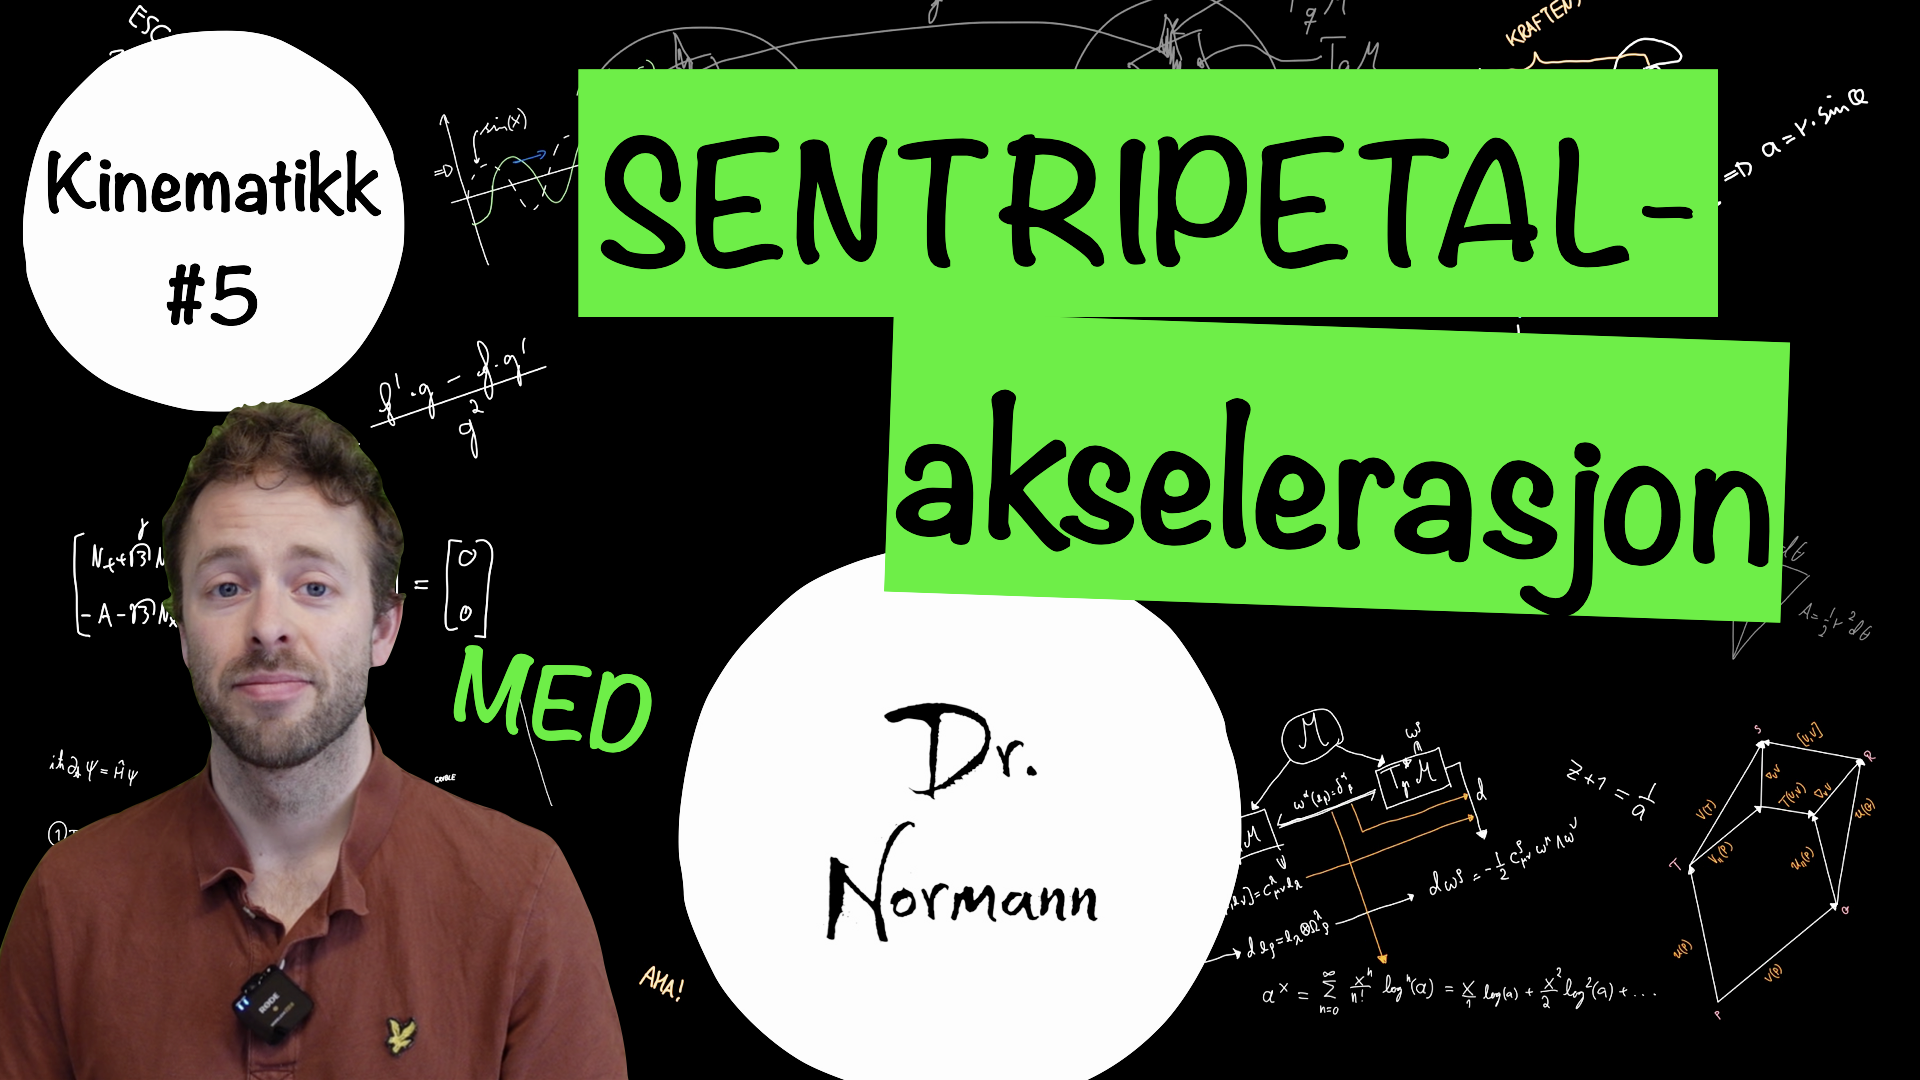
\includegraphics[width=3.6cm]{Images/YouTubeLenker/YT_Sentripetalakselerasjon.png}};
\node[anchor=north west] at (thumb.south west) {
\includegraphics[width=1.2cm]{Images/YouTubeLenker/Icon.png}};
\end{tikzpicture}%
}}%
\end{wrapfigure}
Sentripetalakselerasjonen peker alltid mot sentrum av sirkelen, selv om objektet hele tiden beveger seg langs kanten av sirkelen. Dette er en viktig idé å forstå når vi ser på bevegelse i sirkulære baner. Men... hva om bilen også øker farten sin langs sirkelbanen, og ikke bare endrer retning? I det tilfelel vil bilen både ha en akselerasjon inn mot sentrum (sentripetalakselerasjonen) og en akselerasjon i kjøreretningen (tangentialakselerasjonen). Den totale akselerasjonsvektoren kan da skrives som en sum av disse to komponentene:
\[
\vec{a} = \vec{a}_\perp + \vec{a}_\parallel,
\]
hvor \( \vec{a}_\perp \) er sentripetalakselerasjonen og \( \vec{a}_\parallel \) er tangentialakselerasjonen. I dette faget skal vi ikke se på slike tilfeller, men det er greit å ha sett sammenhengen. 


\exm{Bil i rundkjøring}{%
En bil kjører gjennom en rundkjøring med konstant fart $v = \SI{36}{\kilo\metre\per\hour}$ og radius $r = \SI{20}{\metre}$.
Hva er sentripetalakselerasjonen til bilen?
}

\svar{%
\noindent
Vi starter med å gjøre om farten til \si{\metre\per\second}:
\[
    v = \SI{36}{\kilo\metre\per\hour} = \SI{10}{\metre\per\second}
\]
Deretter bruker vi formelen for sentripetalakselerasjon:
\[
    a_\perp = \frac{v^2}{r} = \frac{(\SI{10}{\metre\per\second})^2}{\SI{20}{\metre}}
    = \frac{\SI{100}{\metre\squared\per\second\squared}}{\SI{20}{\metre}}
    = \doubleunderline{\SI{5}{\metre\per\second\squared}}
\]
Akselerasjonen peker hele tiden inn mot sentrum av rundkjøringen, selv om bilen beveger seg fremover.
}

\oppgave{Sykkel i sving}{%
En syklist kjører gjennom en sirkulær sving med radius $r = \SI{12}{\metre}$ og konstant fart $v = \SI{5.4}{\kilo\metre\per\hour}$.
\begin{enumerate}[a)]
    \item Gjør om farten til \si{\metre\per\second}.
    \item Finn sentripetalakselerasjonen til syklisten.
    \item Hva skjer med sentripetalakselerasjonen om syklisten dobler farten? Forklar svaret.
\end{enumerate}
}


\subsection{Omløpstid}
Når vi snakker om legemer som har periodisk bevegelse, slik som en satelitt rundt jorda, en planet eller en drill i en borerigg, så er det praktisk å definere begrepet \textit{periode}, $T$, også kalt \textit{omløpstid}. Dette er rett og slett tiden brukt på ett omløp (én runde), Det viser seg at vi nå kan skrive om uttrykket for sentripetalakselerasjonen ved hjelp av omløpstiden. Farten i konstant sirkelbevegelse må nesten kunne uttrykkes som avstanden rundt sirkelen (omkretsen) delt på tiden det tar å fullføre ett omløp, altså $T$. Vi får
\[
v = \frac{2\pi r}{T}.
\]
Ved å sette dette uttrykket for $v$ inn i formelen for sentripetalakselerasjon, får vi
    \begin{align}
        \colorbox{black!7}{$\displaystyle a_\perp = \dfrac{4\pi^2 r}{T^2}$}
    \end{align}


\exm{Jorda rundt sola}{%
Jorda beveger seg i en tilnærmet sirkulær bane rundt sola med gjennomsnittlig radius $r = \SI{1.496e11}{\metre}$ og omløpstid $T = \SI{365.25}{\day}$.
Hva er den gjennomsnittlige sentripetalakselerasjonen jorda opplever?
}

\svar{%
\noindent
Vi starter med å gjøre om omløpstiden til sekunder:
\[
    T = \SI{365.25}{\day} \cdot \frac{\SI{24}{\hour}}{\SI{1}{\day}} \cdot \frac{\SI{3600}{\second}}{\SI{1}{\hour}}
    = \SI{3.156e7}{\second}
\]
Deretter setter vi inn i formelen for sentripetalakselerasjon:
\[
    a_\perp = \frac{4\pi^2 r}{T^2}
    = \frac{4\pi^2 \cdot \SI{1.496e11}{\metre}}{\left(\SI{3.156e7}{\second}\right)^2}
    = \doubleunderline{\SI{5.93e-3}{\metre\per\second\squared}}
\]
Dette er omtrent $6.1\cdot10^{-3}$ ganger tyngdeakselerasjonen $g$. Selv om akselerasjonen er svært liten, er det nok til å holde jorda i bane rundt sola — fordi tyngdekraften virker over en enorm avstand.
}

\oppgave{Sirkelbevegelse og omløpstid}{%
Månens gjennomsnittlige avstand fra jorda er $r = 3.84 \cdot 10^8\,\si{\metre}$, og omløpstiden er $T = 27.3\,\textrm{dager}$.
\begin{enumerate}[a)]
    \item Gjør om omløpstiden til sekunder.
    \item Finn sentripetalakselerasjonen månen opplever ved hjelp av formelen $a_\perp = 4\pi^2 r / T^2$.
    \item Beregn månens banehastighet $v = 2\pi r / T$ og verifiser svaret ved å bruke $a_\perp = v^2/r$.
\end{enumerate}
}
